\documentclass{article} % For LaTeX2e
\usepackage{nips13submit_e,times}
\usepackage{hyperref}
\usepackage{url}
\usepackage{authblk}
\usepackage{graphicx}
\usepackage[numbers]{natbib}
\usepackage{amsmath}
\usepackage[normalem]{ulem}
\usepackage{subcaption}

%\documentstyle[nips13submit_09,times,art10]{article} % For LaTeX 2.09

\begin{document}

\title{Applying Deep Learning to predict Bracketology for NCAA's March Madness
\author[1]{Loyzer, Mark \texttt{loyzer@cs.toronto.edu}}
\author[2]{Seward, Neil \texttt{neil.seward@uoit.ca}}
\affil[1]{University of Toronto}
\affil[2]{University of Ontario Institute of Technology}
}





\newcommand{\fix}{\marginpar{FIX}}
\newcommand{\new}{\marginpar{NEW}}

\nipsfinalcopy % Uncomment for camera-ready version

\maketitle

\section{Introduction}
This project focuses on predicting the bracketology for NCAA's March Madness tournament.
We leverage the dataset from Kaggle's online competition \citep{kagglecompetition}.
Parsing the data and constructing relevant features is one of the main efforts in this project as all the data provided is.
The data comes in two forms: detailed and compact, where compact is a subset of the features in detailed.
The ground-truth labels are stored as another feature in the data and so can easily be obtained.
For each example, the a subset of the features can remain to comprise the feature vector; however, additional features are added and discussed in section~\ref{sec:data-features}.


The task of predicting the all-but-first bracketology is complex: the first round (initial seedings are provided to you, and you must predict the winners of the subsequent rounds until only one team remains and is crowned champion.
For the second round there will be $2^{32}$ possible outcomes since there are 64 teams in the first round.
Then $2^{16}$, \dots, $2$ possibilities for each subsequent round.
Since each round depends on the results of the previous there are $\prod_{i=1}^{\log(32)} 2^{2^{i}} = \prod_{i=1}^{\log(32)} 4^{i} = 4^{\Sigma_{i=1}^{\log(32)} i} = 4^{15}$ possible outcomes.
 The odds of predicting a perfect bracket are poor with the probability being $\frac{1}{4^{15}} \approx 9.3132257e^{-10}$.
So, let the odds forever be in our favour.


To generate competitive performance, we considered a variety of deep learning models which exploit different feature representations.
We attempt both the detailed and compact feature sets as well as additional hand-crafted and learned features as well.
Since the application of deep learning to predicting tournament bracketology is new (we could not find any articles to people who have tried this before) we experiment with a few different deep learning models to see which performs/generalizes best.
The models are described in section~\ref{sec:models}.
We describe the setup, performance, results, and summarize the investigation for each of the techniques.


\section{Background and Related Work}
\label{sec:background-related-work}

\textbf{Brief overview of previous models.}
Many of the current and past contestants in Kaggle's competition \citep{kagglecompetition} use some very primitive models like linear or logistic regression.
While others have used statistical measures to quantify (or rank) how good a team is.
Some of these measures are by a Winning Index but the more common approach was to use ELO \citep{elo} and so the winner was the team that had the better score using a direct comparison between the two teams.
Some of the early attempts were to compute these metrics or even an offensive and defensive rating (on the same scale) and compute a linear combination of the two team's offensive and defensive ranking and predict the team that matches up best against each other.
Some ensemble methods were tried using Adaboost and decision tree stumps with some succes.
Starting in about 2015 some people started using neural networks, though the techniques I saw were player based models instead of team where players are categorized based on the role positions in basketball, and the final game roster is based on the players that played the most during the season.

\textbf{Investigating the success of past winners.}
The winner in 2013 used represented a team as a vector of the 5 players on a court at any given timeEach position would be given a real number which indicated how good that team was at that position for both offense and defense.
Predicted scored were computed by taking the dot product between oppossing vectors (offsense with defense) and the predicted winning team would be the one with the larger predicted score.
The optimization/learning was in the determining the values for the offensive and defensive vectors.
A squared error cost function was used with a convex optimization algorithm.
The winners in 2014 used a margin-of-victory model which predicted the difference in score between the two teams and chose the winning team with the positive margin.
Their model was updated as games completed during the tournament which helped account for any inconsistencies or potentialy exceptional situations that could be inferred from score (for example, a team's best player being injurred and out after the first two quarters in a round 1 game).
In 2015 the winner took a bayesian approach incorporating his experience as a sports analyst as the priors in a Bayesian classifier \citep{kaggle2015winner}.
In 2016, the winners initially tried using Adaboost (which is a way to combine multiple weak classifiers into one final classifier) but received poor results \citep{kaggle2016winner} and decided to opt for a logistic regression classifier with random forests (which is also an ensemble learning method).
Random forests combine several decision tree classifiers to predict the target usually using a weighted mean over all decision trees.


\textbf{Survey of models for game prediction.}
The dissertation by \citet{cao2012sports} investigates using a simple logistic classifier, neural networks, support vector machines, and naive Bayes with performance being in that order.
They also consider an engineered feature of the past 10 home/road games but distinguish between a home and away game.
They also consider external features like game schedule (home vs away game is considered an external feature as well).

\textbf{Traditional measures are inadequate.}
The paper by \citet{bashuk2012using} disqualify using traditional ranking methods such as Average Scoring Margin (ASM) and Ratings percentage Index (RPI) due to their myopic view of considering only scores in past games to predict future game outcomes.
\citet{bashuk2012using} investigate cumulative win probabilities over the duration of a game to measure both the team and each player's individual performance.
They then use 5 years of past game data to generate a ``Win Probability Index" (WPI) metric which outperforms ASM and RPI in predicting NCAA basketball games.
This paper shows the advantages of using indirect but correlated features (with respect to winning) and invokes the question as to which is more imporant: less data with more (but hopefully relevant) features or more data with only a subset of the features.
This will be evaluated as the compact and detailed datasets provided begin with


\textbf{NNs for predicting soccer matches.}
\citet{huang2010neural} predict football games' win rate between two teams according to their previous stage's statistical data.
The predictions were on 2006 World Cup Football games.
The inputs were transformed to relative ratios between the teams for each game.
They achieved 76.9\% prediction accuracy when draw (tie) games were excluded using a simple one-hidden layer network with 11 hidden nodes.

\textbf{NNs for predicting a variety of sports.}
\citet{mccabe2008artificial} predict game outcomes for the Australian National Rugby League (NRL), the Australian Football League (AFL), Super Rugby (Super 12 and Super 14) and English Premier League football (EPL).
They use a set of handcrafted features sport-independent (like score, ``performance" metrics, rankings, location of game, etc) allowing for one model to be used across different sports.
They achieve prediction rates as low as $58.9\%$ in EPL and as high as $75.4\%$ in Super Rugby.


\textbf{Predicting NBA games using NNs.}
\citet{loeffelholz2009predicting} use a few neural network approaches: a traditional feed-forward NN, a traditional radial basis network, and two other radial basis networks, a probabilistic NN, and a generalized regression NN.
They also try an ensemble approach using each of the NNs output to produce a final classification.
Their average results across several validation sets was between $69\%$ and $71\%$ across all NNs.




\section{Data}
\label{sec:data}

In this task we take on the challenge of predicting the winner between two teams in a game.
In its most general case you can consider the training input to be of the form: [[vector for team1], [vector for team2], [vector of comparative stats]], and so there is some natural \textit{symmetry} within each training example.
Namely we could have given the input as [[vector for team2], [vector for team1], [vector of comparative stats]] as well and the target output would be either be identical or reflexive depending on what the output layer represents, but ultimately the target output would refelect which team won.
Due to this symmetry we actually do create both training examples during the data-collection process.
This doubles our data size and allows the computational models to be more robust in predicting games where we won't be necessarily given some predefined structure (like alphabetical ordering by team name as an example).

\subsection{Setup}
\label{sec:data-setup}

There are two data sets we explored.
The compact and detailed data sets provided by Kaggle \citep{kagglecompetition}.
Each file and their description is below.
Before evaluating the models one thing to note is that the compact vs detailed vary in the number of data examples each have.
Compact results have been aggregated from 1985 to present, while detailed results have only been aggregated from 2003 to present.
This leaves an interesting question as to is more data with fewer features a better predictor than less data but more features.
Clearly there is some tradeoff (maybe some of the detailed features are noise and not relevant predictors but without more data the model is not able to learn this).

The results datasets (RegularSeasonCompactResults, RegularSeasonDetailedResults, TourneyCompactResults, and TourneyDetailedResutls) are used in the intuitive sense: they comprise the basis for the examples to train and evaluate the predictor model.
The daynum feature was used to actually merge the results into one dataset.
This was done because we also constructed two handcrafted features which we call the hot-streak and rival-streak (see section~\ref{sec:data-features-handcrafted}).
The hot-streak is the win/loss for a team in the past X games, and the rival-streak is the win/loss for the past Y games for the current matchup.

RegularSeasonCompactResults\\
This file identifies the game-by-game results for 32 seasons of historical data, from 1985 to 2015. Each year, it includes all games played from daynum 0 through 132 (which by definition is ``Selection Sunday," the day that tournament pairings are announced). Each row in the file represents a single game played.


RegularSeasonDetailedResults\\
This file is a more detailed set of game results, covering seasons 2003-2016. This includes team-level total statistics for each game (total field goals attempted, offensive rebounds, etc.) The column names should be self-explanatory to basketball fans (as above, ``w" or ``l" refers to the winning or losing team):


TourneyCompactResults
This file identifies the game-by-game NCAA tournament results for all seasons of historical data. The data is formatted exactly like the RegularSeasonCompactResults data. Note that these games also include the play-in games (which always occurred on day 134/135) for those years that had play-in games.

TourneyDetailedResults\\
This file contains the more detailed results for tournament games from 2003 onward.


Seasons\\
This file identifies the different seasons included in the historical data, along with certain season-level properties such as the season's year and day number, as well as how the regions are categorized for tournament play.

"season" - indicates the year in which the tournament was played.

"dayzero" - tells you the date corresponding to daynum=0 during that season. All game dates have been aligned upon a common scale so that the championship game of the final tournament is on daynum=154. Working backward, the national semifinals are always on daynum=152, the "play-in" games are on days 134/135, Selection Sunday is on day 132, and so on. All game data includes the day number in order to make it easier to perform date calculations. If you really want to know the exact date a game was played on, you can combine the game's "daynum" with the season's "dayzero". For instance, since day zero during the 2011-2012 season was 10/31/2011, if we know that the earliest regular season games that year were played on daynum=7, they were therefore played on 11/07/2011.

"regionW/X/Y/Z" - by convention, the four regions in the final tournament are always named W, X, Y, and Z. Whichever region's name comes first alphabetically, that region will be Region W. And whichever Region plays against Region W in the national semifinals, that will be Region X. For the other two regions, whichever region's name comes first alphabetically, that region will be Region Y, and the other will be Region Z. This allows us to identify the regions and brackets in a standardized way in other files. For instance, during the 2012 tournament, the four regions were East, Midwest, South, and West. Being the first alphabetically, East becomes W. Since the East regional champion (Ohio State) played against the Midwest regional champion (Kansas) in the national semifinals, that makes Midwest be region X. For the other two (South and West), since South comes first alphabetically, that makes South Y and therefore West is Z. So for this season, the W/X/Y/Z are East,Midwest,South,West.



Teams\\
This file identifies the different college teams present in the dataset. Each team has a 4 digit id number.


\subsection{Features}
\label{sec:data-features}

The data provided was on a per-game basis.
The features per example were temporally parochial to a specific game, and the teams were assigned the `w' or `l' metrics based on if they won or lost, respectively.
With this, it is very easy to determine who wins each game, either read the `wteam' feature or compare the twot eams' scores.
However, for prediction tasks we will not be given the metrics on a game until that game is done (at which time there is no purpose in predicting).
From these per-game data instances we need to come up a feature vector that provides pertinent information to predict the current game winner \textit{based on all of the past games} (or all of the data up prior to that game assuming the data is ordered chronologically).
Therefore, processing the data is an entirely different task and requires significant effort in determining:

\begin{enumerate}
  \item \label{itm:features-pertinent} Which features are pertinent to predict future game outcomes
  \item \label{itm:features-aggregate} What aggregation methods should be used to summarize the values of the features across time
  \item \label{itm:features-horizon} What temporal horizon should be used when aggregating the features?  Should only the current season statistics be used, or the entire lifetime, or the past X games?
\end{enumerate}

We will discuss each of these in turn, but first \label{itm:features-pertinent} will be discussed with respect to the two datasets (compact vs detailed).


\subsubsection{Compact}
\label{sec:data-features-compact}

The compact dataset includes the features below.
The features we keep track of are not striked out, while the features that are \sout{striked out} are ones that are included in the dataset but were not used as input towards the predictive model.
Also, there is a convention that a ``w" or ``l" that precedes a feature represents the value of that feature for the winning and losing team, respectively.

\begin{description}
  \item[\sout{season}] - this is the year of the associated entry in seasons.csv (the year in which the final tournament occurs)
  \item[\sout{daynum}] - this integer always ranges from 0 to 132, and tells you what day the game was played on. It represents an offset from the ``dayzero" date in the ``seasons.csv" file. For example, the first game in the file was daynum=20. Combined with the fact from the ``season.csv" file that day zero was 10/29/1984, that means the first game was played 20 days later, or 11/18/1984. There are no teams that ever played more than one game on a given date, so you can use this fact if you need a unique key. In order to accomplish this uniqueness, we had to adjust one game's date. In March 2008, the SEC postseason tournament had to reschedule one game (Georgia-Kentucky) to a subsequent day, so Georgia had to actually play two games on the same day. In order to enforce this uniqueness, we moved the game date for the Georgia-Kentucky game back to its original date.
  \item[\sout{wteam}] this identifies the id number of the team that won the game, as listed in the ``teams.csv" file. No matter whether the game was won by the home team or visiting team, ``wteam" always identifies the winning team.
  \item[wscore] this identifies the number of points scored by the winning team.
  \item[\sout{lteam}] this identifies the id number of the team that lost the game.
  \item[lscore] this identifies the number of points scored by the losing team.
  \item[\sout{numot}] this indicates the number of overtime periods in the game, an integer 0 or higher.
  \item[\sout{wloc}] this identifies the ``location" of the winning team. If the winning team was the home team, this value will be ``H". If the winning team was the visiting team, this value will be ``A". If it was played on a neutral court, then this value will be ``N". Sometimes it is unclear whether the site should be considered neutral, since it is near one team's home court, or even on their court during a tournament, but for this determination we have simply used the Kenneth Massey data in its current state, where the ``@" sign is either listed with the winning team, the losing team, or neither team.
\end{description}




\subsubsection{Detailed}
\label{sec:data-features-detailed}
The features in the detailed version of the data supersets the compact features.
The additional features (not included in compact) are the following where, again, w and l represent the statistic for the winning and losing team respectively and only the winning team statistics are shown for conciseness.
All new features are included in the predictive model (if the detailed dataset is used as we compare the predictiveness of the two datasets separately).

\begin{description}
  \item[wfgm] field goals made
  \item[wfga] field goals attempted
  \item[wfgm3] three pointers made
  \item[wfga3] three pointers attempted
  \item[wftm] free throws made
  \item[wfta] free throws attempted
  \item[wor] offensive rebounds
  \item[wdr] defensive rebounds
  \item[wast] assists
  \item[wto] turnovers
  \item[wstl] steals
  \item[wblk] blocks
  \item[wpf] personal fouls
\end{description}


\subsubsection{Handcrafted Features}
\label{sec:data-features-handcrafted}

There are two handcrafted features that we chose to incorporate into out feature-set.
We investigate the use of each of these employing a leave-one-out-like evaluation which investigated the affect of adding each of the features independent of each other.

The first handcrafted feature is called a team's ``hot streak".
Hot streak is the win/loss vector for a team in any given season.
To resolve issues where a team has not played many like (for example the first game of each season) we defined the win/loss vector to be a vector with values in the domain ${-1, 0, 1}$, where -1 represents loss, 0 represents not played, and 1 represents win.
This way for any unplayed games we can pad the hot streak vector with 0s and fill in the appropriate games with a -1 or 1.
So, for early season games this feature does not provide much information.

The second handcrafted feature is called a team's ``rival streak" with respect to another team (referred to as the rival). The win/loss vector also uses the domain ${-1, 0, 1}$ with the same meanings as in the hot streak vector.
What is interesting is that, intuitively, it complements hot streak by looking back into the an arbitrary horizon in the past and incorporates the X most recent games (ands pads with 0s if there are less than X games).
But rival streak goes beyond the current season and looks at the most recent $\min(X, \text{number games played against rival team in history})$.
So when hot streak provides little to no information there is still a good chance that rival streak will have some data that the model can leverage (obviously there is nothing we can do for the birth range of the dataset).

As a test-bed we evaluated the impact of hot streak and rival streak in several model architectures.
The results are in section~\ref{sec:results}.



\subsection{Team Snapshot}
\label{sec:data-team-snapshot}

Each input model takes in each team's ``snapshot" which is a feature vector of the how the team has performed in each of the various feature dimensions in the past.
A team's snapshot is a vector containing the features that are not \sout{striked out} in sections \ref{sec:data-features-compact} and \ref{sec:data-features-detailed} depending on whether the compact or detailed datasets are used.

\subsection{Feature Aggregation}
\label{sec:feature-aggregation}

There are many ways to aggregate the features.
Simple methods such as a cumulative total, mean, or applying some distribution which favours recent values and discounts older results (making them less influential or obsolete) are all possible.
For simplicty we chose to use the mean.
This choice came down to picking a simple one that we believed would still be reflective in a team's ability.
Although picking an optimal aggregation method would require many comparisons it seems as though the optimal aggregation techniqe will depend on the feature vector's horizon which determines how far in the past we consider as having influence on a game happening at present.
With mean being the aggregation method, we still need to define the horizon to consider on examples which says how many past games will be considered to compute the feature vector to predict the outcome of a new game.

\subsection{Feature Horizon}
\label{sec:feature-horizon}

A feature vector's temporal horizon is a quantiative measure of how far back to look at past data to compute the values of the feature vector.
Possibilities include a specific number of previous games, the current season, the entire life-data, a specific amount of days or months or seasons, etc.
There are many choices of which we decided to use a team's entire life-data.

In hindsight: Considering that a team's seasonal data is chosen as a feature horizon, it seems as though there is potential to improve this by providing a better initialization from previous season(s) rather than a 0-default.
Because the horizon was only a season, we believe that temporally weighted initializations would have been better but not have had signifcant differences because the number of examples that influence the result are minimal (maximum is around 40 games per season including tournament games).

Though with the more data samples it seems more intuitive in using an aggregation method which applies more weight to recent examples and discounts older ones seems to be the ``best" choice for an aggregation technique.

Note that the feature horizon we chose applies only to the features defined in sections \ref{sec:data-features-compact} and \ref{sec:data-features-detailed} and not the handcrafted features in section~\ref{data-features-handcrafted}


\section{Input Output Architectures}
\label{sec:io-architectures}

The basic model consists of input and output.
We investigate two different input/output combinations and comment on the reasoning behind using each one.
The models below vary on how the input and/or output layer is modelled and interpreted.


The input examples are constructed by processing the data described in section~\ref{sec:data}.
We investigate using both the detailed (section~\ref{sec:data-features-detailed}) and compact (section~\ref{sec:data-features-compact}) data sets.
Each I/O architecture contain the basic ``team snapshot" which is described in section~\ref{sec:data-team-snapshot}.

\subsubsection{Predicting Winning Team ID}
\label{sec:io-architectures-winning-team-id}

This model asked to output the winning team's id given the input training examples.
For this, it should be expected to be given each team's id as part of the input and then output one of the team's id the model believe will win.
Recall that a team's id is given as a one-hot encoding, so if there are T teams then the vector for a team id will be a T-dimensional vector with a single 1 in one of the cells.

So, an example of a single input is:

% Math mode for matrix
\[
\begin{bmatrix}
  \begin{Bmatrix}
    \text{one hot encoding for team1's id}
  \end{Bmatrix}
  \\
  \begin{Bmatrix}
    \text{one hot encoding for team1's feature snapshot}
  \end{Bmatrix}
  \\
  \begin{Bmatrix}
    \text{one hot encoding for team2's id}
  \end{Bmatrix}
  \\
  \begin{Bmatrix}
    \text{vector for team2's feature snapshot}
  \end{Bmatrix}
  \\
  \begin{Bmatrix}
    \text{vector for rival streak wrt team1 (win means team1 won)}
  \end{Bmatrix}
\end{bmatrix}
\]

which will be \textit{flattened} into a single row vector in the input matrix.

And the output represents a T-ary classification problem, where T is the number of teams:
\[
\begin{Bmatrix}
  \text{one hot encoding of winning team}
\end{Bmatrix}
\]


The advantages for this model is that we can read the winning team directly from the output layer and that, perhaps, the model can learn additional features between team-pairings.
The ability for the model to output a team that was not even playing the same is prone to more errors than a model that simply predicts a binary classification (team1 either wins or loses).
This additional burden on the model may require more data to simply learn valid outputs given the inputs.
The reason for trying this model is that with each team id as input the model may learn team-specific associations (for example team X always beats team Y); however, team ids could still be used as input to a more appropriate binary classification problem, or the rival streak feature may be sufficient with this as well (though it is not identical).

\subsection{Predicting Win/Loss Vector}
\label{sec:io-architectures-symmetrical}

This is a binary classification model is asked to output one of the following two vectors: $\begin{Bmatrix} 1, 0 \end{Bmatrix}$ or $\begin{Bmatrix} 0, 1 \end{Bmatrix}$ representing that either the first or second team will win, respectively.
The learned predictive model will hopefully learn a probability distribution of each of the two teams winning, then the max output signal can be computed and the winner determined.
For the model, we no longer require the input to include either team's unqiue id as the output is relative to the ordering of the input.
The intuitive reasoning for this is that the team's themselves are probably not a significant indicator for winning or losing, but their seasonal and lifetimes statistics are (relevant indicators).
This also removes the requirement for the model to learn that the output has valid outputs according to the input.
Invalid outputs are no longer possible.
Furthermore, this reduces the memory burden during learning as we have a reduced the feature size.
Since there are approximately 350 different teams, this reduces the feature dimension by $2 * 350 = 700$ (even though most of these features are 0).

So, an example of a single input is:

% Math mode for matrix
\[
\begin{bmatrix}
  \\
  \begin{Bmatrix}
    \text{vector for team1's feature snapshot}
  \end{Bmatrix}
  \\
  \begin{Bmatrix}
    \text{vector for team2's feature snapshot}
  \end{Bmatrix}
  \\
  \begin{Bmatrix}
    \text{vector for rival streak wrt team1 (win means team1 won)}
  \end{Bmatrix}
\end{bmatrix}
\]

which will be \textit{flattened} into a single row vector in the input matrix.

And the output would be
\[
\begin{cases}
  \begin{Bmatrix} 1, 0 \end{Bmatrix}, & \mbox{ if the first input team is predicted to win}\\
  \begin{Bmatrix} 0, 1 \end{Bmatrix}, & \mbox{ if the second input team is predicted to win}
\end{cases}
\]




\section{Models}
\label{sec:models}
In this section we present an inital logistic regression classifier that we use as a baseline model and then present the deep learning architectures that were experimented with to predict game outcomes.


\subsection{Logistic}
\label{sec:model-logistic}

As our baseline model we decided to use a logistic classifier and tested it with different the different features discussed above.
For our baseline we only investigate the binary classification problem.

The logistic classifier is defined as,
\begin{equation} 
\label{eqn:logistic}
p(x) = \frac{1}{1 + \mathrm{e}^{-\theta x}}
\end{equation}
where $\theta$ are the learned parameters and $x$ is the input vector.


\subsection{Neural Network Architectures}
\label{sec:nn-architectures}

We experimented on a single hidden layer fully-connected neural network (multi-layer perceptron [MLP]) and investigated the highest performing data-configuration on a 2 layer MLP.

To be specific, each fully connected layer is used at the output of the neural network. No convolutions are used as there is not a spatial correlation between the metrics.
Therefore, the model is as follows:

\begin{gather}
{h_{j}}^l = \sigma({w_{i,j}}^{l} {h_{i}}^{l-1} + {b_j}^l) 
\end{gather}

where $h^l_{i,j,n}$ is the (i,j)-th indexed output in the l-th layer in channel n, while $w_{a,b,m,n}$ is a weight in the convolution layer, and $b_n$ the bias value for the n-th output layer. 


Various configurations (discussed above) using MLPs are instantiated using the Google TensorFlow package.
The network is then optimized using the built in AdamOptimizer, with cross entropy as the loss/cost function to be minimized:

\begin{gather}
J(w) = - \sum_{i}{\sum_{k=0}^{9}{t^{(i)}_k}log(y_k(x^{(i)}))}
\end{gather}

where t are the one-hot targets, and y is the the output vector of the final multi-class softmax function. 

Mini-batch training is used to train the neural networks, with 128 input samples per batch.
These mini-batches are selected at random with replacement from the sample set.

Through experimentation, it is found that initializing the weights and biases with a Gaussian distribution of zero mean and standard deviation of 0.01 resulted in training sequences with gradients that do not explode early in the training process. 

For each neural network configuration, training is done until the validation error (evaluated every 1000 epochs) becomes roughly constant.
The weights from the iteration where the validation error is minimum are used to obtain an evaluation for the final test set evaluation which are discussed in section~\ref{sec:results}.




\section{Results}
\label{sec:results}

For all graphs, the we plot the training loss and accuracy after each batch and plot the validation loss and accuracy 50 times during the entire training process.
The data was partitioned as follows: training: $80\%$, validation: $10\%$, and testing: $10\%$.


Learning rate: $1e^{-4}$\\
Batch size: 128\\
Hot-Streak Length: 10\\
Rival-Streak Length: 10\\


All models are evaluated on both the Compact and Detailed datasets and we look at the accuracy and cross entropy loss for the various curves.

Since Tensorflow does not place the legend within the graph, the legend in figure~\ref{fig:legend} is used for each graph in this section.


\begin{figure}[!htb]
  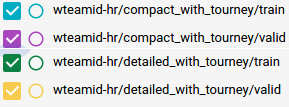
\includegraphics[width=0.5\textwidth]{figures/legend.png}
  \caption{Legend used for all accuracy and cross-entropy charts in this paper.}\label{fig:legend}
\end{figure}

\subsection{Linear Classifier}

For our logisic classifier (our baseline model) the results are shown below.

\begin{figure}[!htb]
  \begin{subfigure}{0.5\textwidth}
    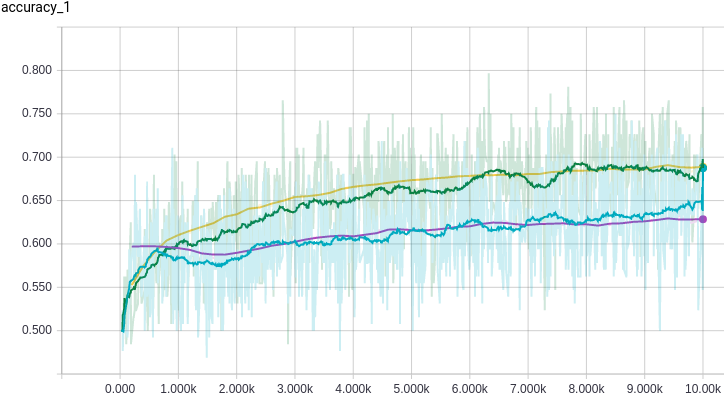
\includegraphics[width=\linewidth]{plots/linear-model/streak-/accuracy.png}
    \caption{Logistic accuracy using no streaks.}\label{fig:linear--accuracy}
  \end{subfigure}
  \begin{subfigure}{0.5\textwidth}
    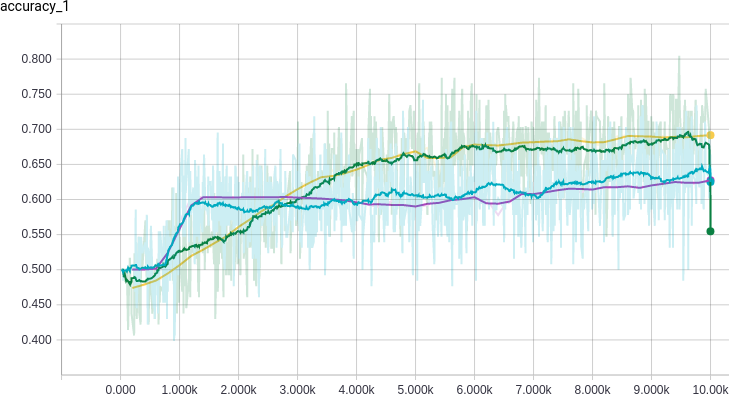
\includegraphics[width=\linewidth]{plots/linear-model/streak-h/accuracy.png}
    \caption{Logistic accuracy using only hot streak.}\label{fig:linear-h-accuracy}
  \end{subfigure}


  \begin{subfigure}{0.5\textwidth}
    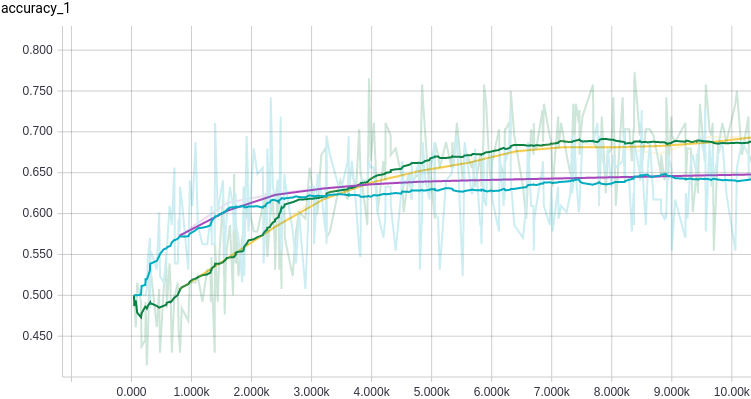
\includegraphics[width=\linewidth]{plots/linear-model/streak-r/accuracy.png}
    \caption{Logistic accuracy using only rival streak.}\label{fig:linear-r-accuracy}
  \end{subfigure}
  \begin{subfigure}{0.5\textwidth}
    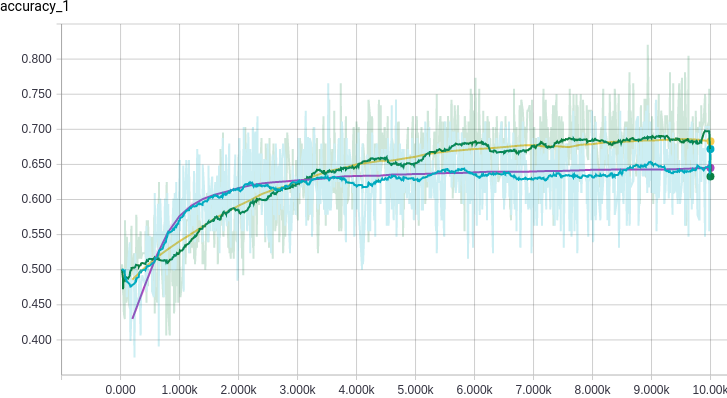
\includegraphics[width=\linewidth]{plots/linear-model/streak-hr/accuracy.png}
    \caption{Logistic accuracy using both hot and rival streaks.}\label{fig:linear-hr-accuracy}
  \end{subfigure}
\end{figure}


\begin{figure}[!htb]
  \begin{subfigure}{0.5\textwidth}
    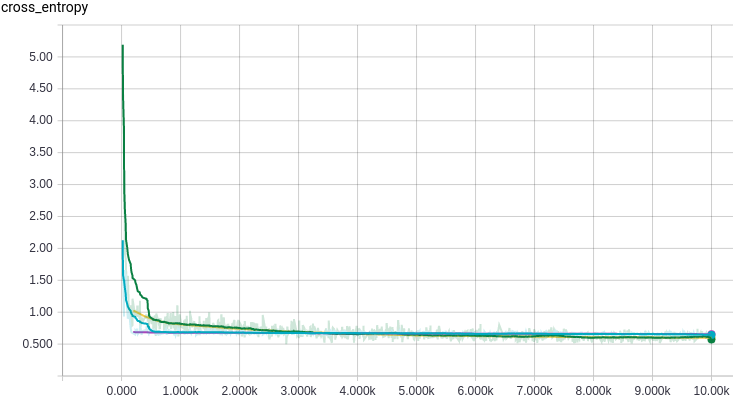
\includegraphics[width=\linewidth]{plots/linear-model/streak-/crossentropy.png}
    \caption{Logistic cross entropy using no streaks.}\label{fig:linear--crossentropy}
  \end{subfigure}
  \begin{subfigure}{0.5\textwidth}
    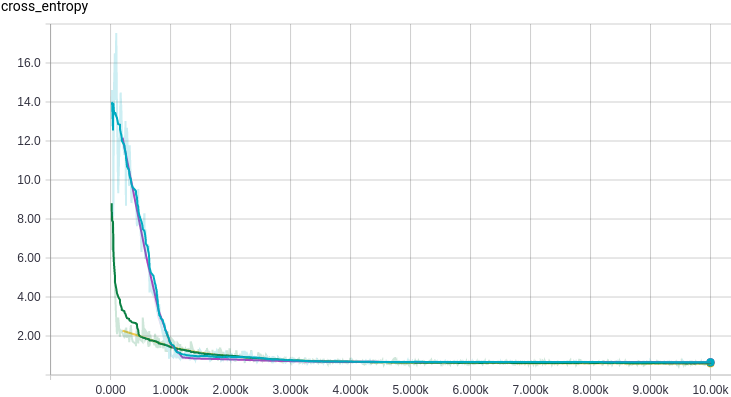
\includegraphics[width=\linewidth]{plots/linear-model/streak-h/crossentropy.png}
    \caption{Logistic cross entropy using only hot streak.}\label{fig:linear-h-crossentropy}
  \end{subfigure}


  \begin{subfigure}{0.5\textwidth}
    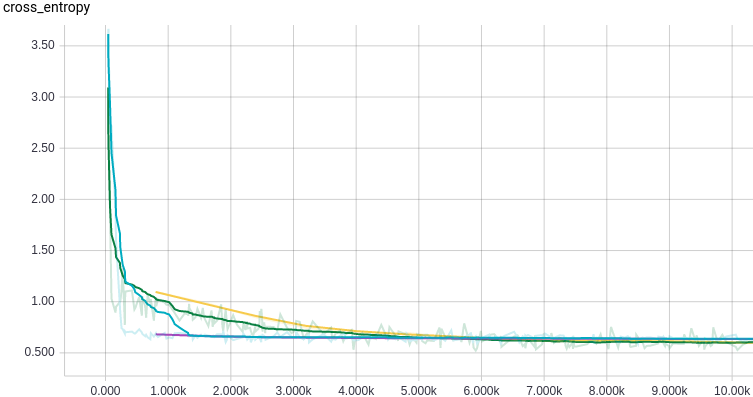
\includegraphics[width=\linewidth]{plots/linear-model/streak-r/crossentropy.png}
    \caption{Logistic cross entropy using only rival streak.}\label{fig:linear-r-crossentropy}
  \end{subfigure}
  \begin{subfigure}{0.5\textwidth}
    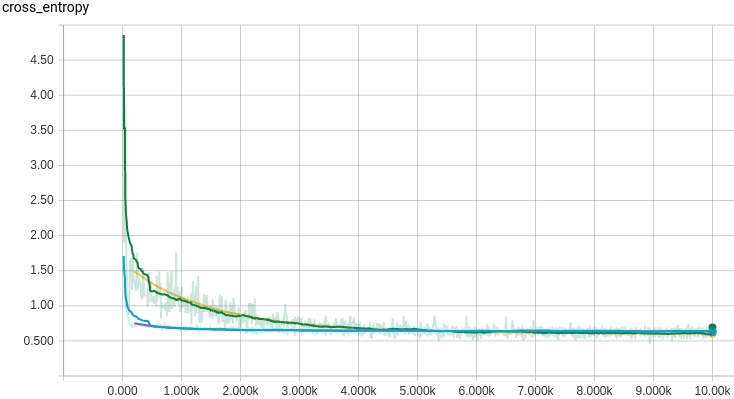
\includegraphics[width=\linewidth]{plots/linear-model/streak-hr/crossentropy.png}
    \caption{Logistic cross entropy using both hot and rival streaks.}\label{fig:linear-hr-crossentropy}
  \end{subfigure}
\end{figure}


We can see that with this model there is not a clear discrepancy between the compact and detailed datasets.
Since all graphs do not overfit on either dataset, this suggests that the model is not flexible enough; however, the significantly poorer performance of the compact-valid curve seem to suggest that overfitting is occuring but the loss function is staying approximately equal.


\begin{table}
\centering
  \begin{tabular}{|l|c|c|c|c|}
  \hline
   & \multicolumn{2}{|c|}{Compact} & \multicolumn{2}{|c|}{Detailed}\\
  Data & loss & accuracy & loss & accuracy\\
  \hline
  Vanilla       & 0.6618 & 0.6096 & 0.6168 & 0.6747\\ 
  +hot streak   & 0.6502 & 0.6098 & 0.6013 & 0.6807\\
  +rival streak & 0.6301 & 0.6407 & 0.6036 & 0.6774\\
  +both streaks & 0.6381 & 0.6411 & 0.6185 & 0.6684\\
  \hline
  \end{tabular}
  \caption{Impact of the handcrafted streak features using a logisitic classifier.}
\end{table}
\label{tbl:test-results-logistic}

Table~\ref{tbl:test-results-logistic} shows that using a simple linear classifier we can reach a $\approx 0.68$ accuracy.
This will act as a baseline performance point to investigate deep learning models on.



\subsection{Predicting Winning Team ID}
\label{sec:results-wteamid}


\begin{figure}[!htb]
  \begin{subfigure}{0.5\textwidth}
    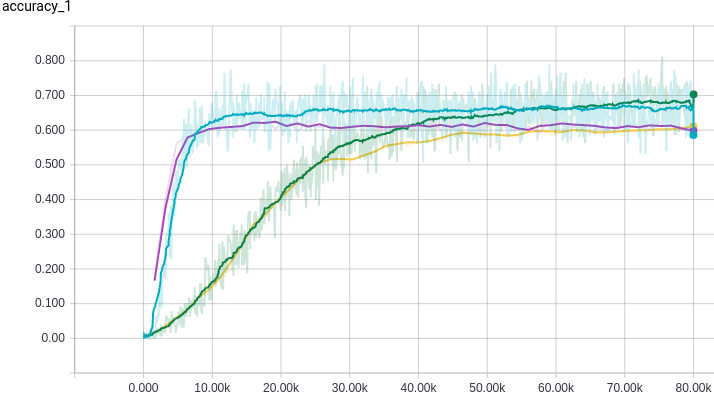
\includegraphics[width=\linewidth]{plots/model1/wteam_onehot/streak-/accuracy.png}
    \caption{Accuracy using no streaks.}\label{fig:wteam-onehot--accuracy}
  \end{subfigure}
  \begin{subfigure}{0.5\textwidth}
    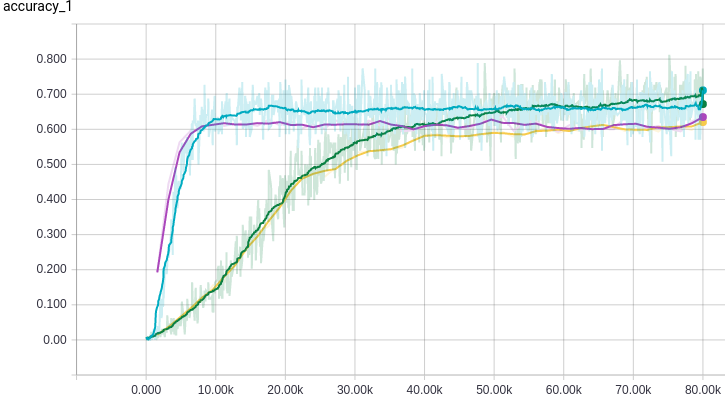
\includegraphics[width=\linewidth]{plots/model1/wteam_onehot/streak-h/accuracy.png}
    \caption{Accuracy using only hot streak.}\label{fig:wteam-onehot-h-accuracy}
  \end{subfigure}


  \begin{subfigure}{0.5\textwidth}
    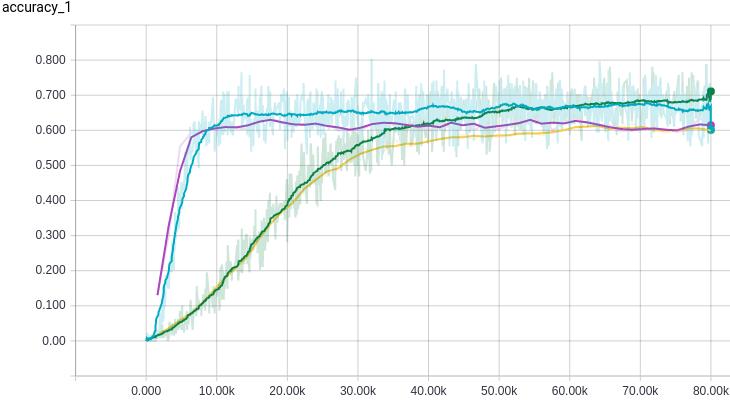
\includegraphics[width=\linewidth]{plots/model1/wteam_onehot/streak-r/accuracy.png}
    \caption{Accuracy using only rival streak.}\label{fig:wteam-onehot-r-accuracy}
  \end{subfigure}
  \begin{subfigure}{0.5\textwidth}
    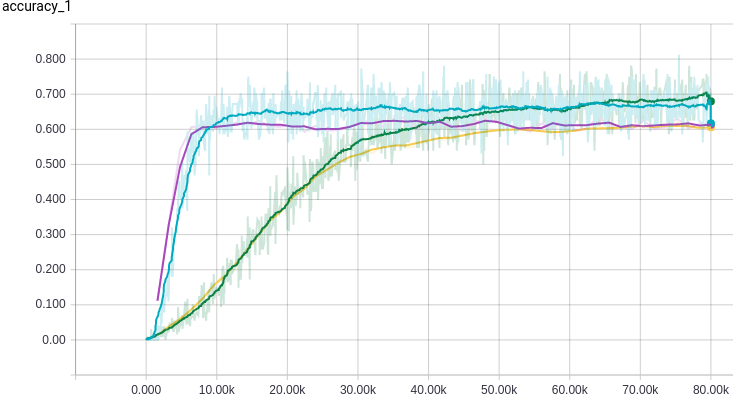
\includegraphics[width=\linewidth]{plots/model1/wteam_onehot/streak-hr/accuracy.png}
    \caption{Accuracy using both hot and rival streaks.}\label{fig:wteam-onehot-hr-accuracy}
  \end{subfigure}
\end{figure}
\label{fig:results-wteamid}


It is evident that all the curves in each of the graphs (in figure~\ref{fig:results-wteamid}) exhibit the same growth shape.
What changes is the x and y values for when each graph plateaus, where x is epoch and y is the accuracy.
These metrics are described table~\ref{tbl:test-results-teamid}.

\begin{figure}[!htb]
  \begin{subfigure}{0.5\textwidth}
    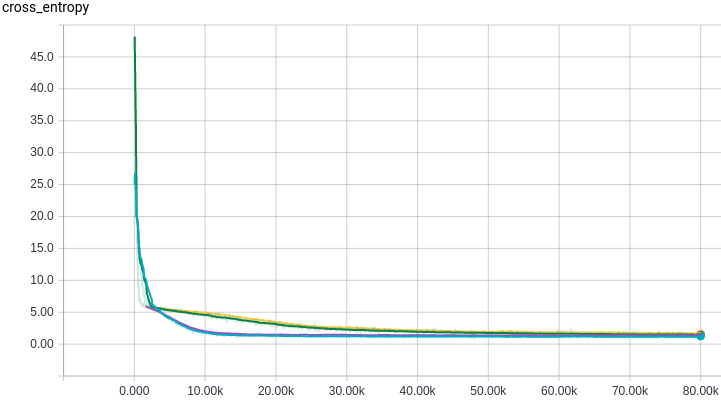
\includegraphics[width=\linewidth]{plots/model1/wteam_onehot/streak-/crossentropy.png}
    \caption{Cross Entropy using no streaks.}\label{fig:wteam-onehot--crossentropy}
  \end{subfigure}
  \begin{subfigure}{0.5\textwidth}
    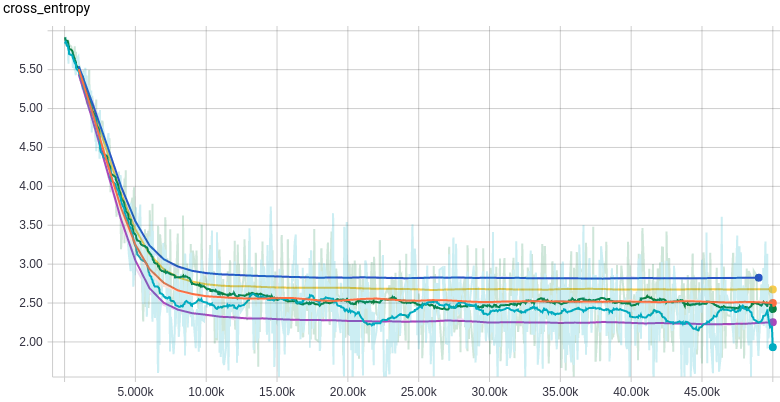
\includegraphics[width=\linewidth]{plots/model1/wteam_onehot/streak-h/crossentropy.png}
    \caption{Cross Entropy using only hot streak.}\label{fig:wteam-onehot-h-crossentropy}
  \end{subfigure}


  \begin{subfigure}{0.5\textwidth}
    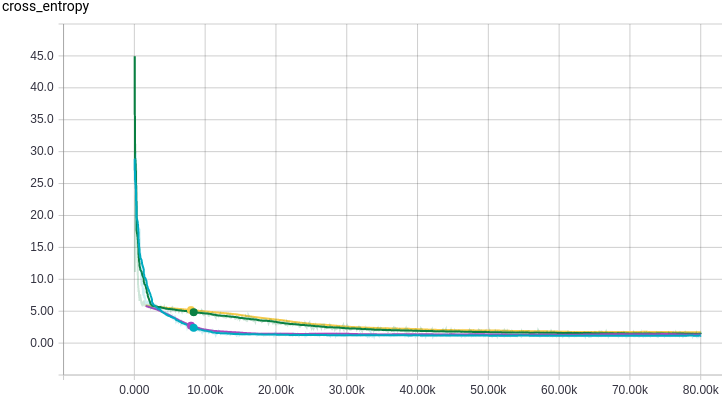
\includegraphics[width=\linewidth]{plots/model1/wteam_onehot/streak-r/crossentropy.png}
    \caption{Cross Entropy using only rival streak.}\label{fig:wteam-onehot-r-crossentropy}
  \end{subfigure}
  \begin{subfigure}{0.5\textwidth}
    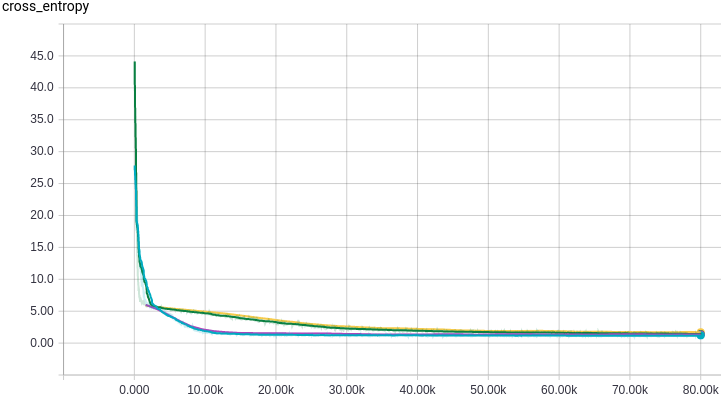
\includegraphics[width=\linewidth]{plots/model1/wteam_onehot/streak-hr/crossentropy.png}
    \caption{Cross Entropy using both hot and rival streaks.}\label{fig:wteam-onehot-hr-crossentropy}
  \end{subfigure}
\end{figure}
For both datasets, the cross entropy loss follows an analogous curve to the accuracy where each curve exhibits the same shape and the training loss drops suddenly right at the end (when the accuracy has a sharp improvement).
There does not seem to be any surprises between the accuracy and cross entropy--that is when the cross entropy drops/rises the accuracy increases/decsreases.


Since the accuracy plateaus and the training data doesn't seem to be overfitting, this is evidence that the model is not complex enough and could better generalize using either additional hidden layers and/or more hidden nodes.
Also since the accuracy is only slightly above $50\%$ for the Vanilla and ``Vanilla + hot streak" models (with the detailed dataset using ``Vanilla + hot streak" predicting below $50\%$, suggests that predicting team id adds a signifcant amount of noise as the model must also learn valid outputs.
Otherwise, this problem should be producing $50\%$ accuracy for a random prediction model, but since we actually require the team id it makes a random prediction model have accuracy $\approx \frac{100}{N}\%$, where $N$ is the number of teams.

\begin{table}
\centering
  \begin{tabular}{|l|c|c|c|c|}
  \hline
   & \multicolumn{2}{|c|}{Compact} & \multicolumn{2}{|c|}{Detailed}\\
  Data & loss & accuracy & loss & accuracy\\
  \hline
  Vanilla       & 1.5510 & 0.5800 & 1.7364 & 0.5866\\ 
  +hot streak   & 1.3892 & 0.6061 & 1.6555 & 0.5957\\
  +rival streak & 1.4716 & 0.5913 & 1.7329 & 0.5899\\
  +both streaks & 1.4760 & 0.5864 & 1.4733 & 0.5919\\
  \hline
  \end{tabular}
  \caption{Impact of the handcrafted streak features on the T-ary classification model.}
\end{table}
\label{tbl:test-results-wteamid}

Table~\ref{tbl:test-results-wteamid} shows that the handcrafted features can have a slight impact--though hot streak seems to be better and the combination of hot streak and rival streak is not as efficient of a feature.
Additionally, the main interest in this section is that the model is able to learn quickly learn that ``valid" output is defined within the features (the outputshould be one of the input team id's).
Since there are approximately 320 teams, a random classifier would have a performance of $\approx \frac{1}{320}$.
However, since the model achieves around $60.6\%$ it is performing signifcantly better than a random model but worse than the binary logisic classifier.




\subsection{Predicting Binary Classification}
\label{sec:results-symmetrical}

With all that has been said it is inefficient to define a T-class classification problem when all we really care about is the relative outcome (did input team1 beat input team2 [or vice-versa]).
This type of question allows us to model a binary classification problem which will be evaluated below.
Because the model does not need to learn team ids it is expected that this model outperforms the previous.

\begin{figure}[!htb]
  \begin{subfigure}{0.5\textwidth}
    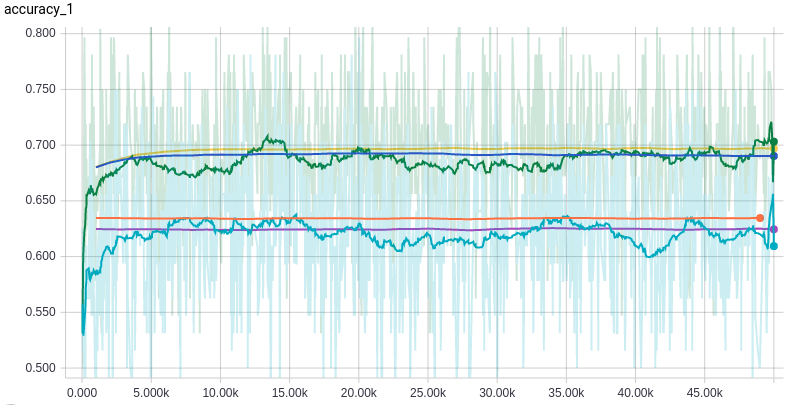
\includegraphics[width=\linewidth]{plots/model1/symmetrical/streak-/accuracy.png}
    \caption{Accuracy using no streaks.}\label{fig:symmetrical--accuracy}
  \end{subfigure}
  \begin{subfigure}{0.5\textwidth}
    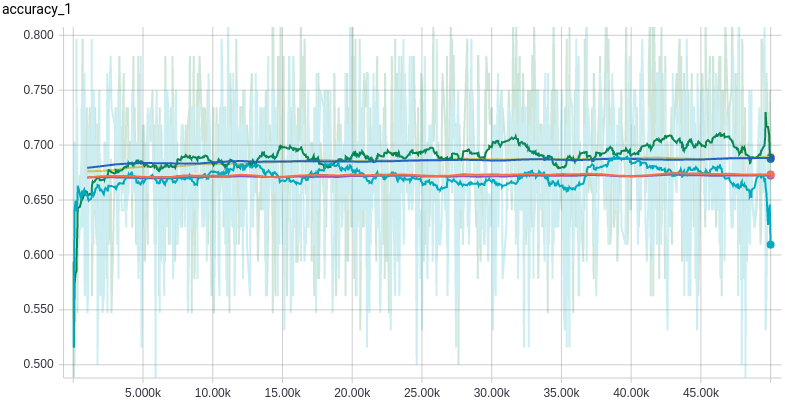
\includegraphics[width=\linewidth]{plots/model1/symmetrical/streak-h/accuracy.png}
    \caption{Accuracy using only hot streak.}\label{fig:symmetrical-h-accuracy}
  \end{subfigure}


  \begin{subfigure}{0.5\textwidth}
    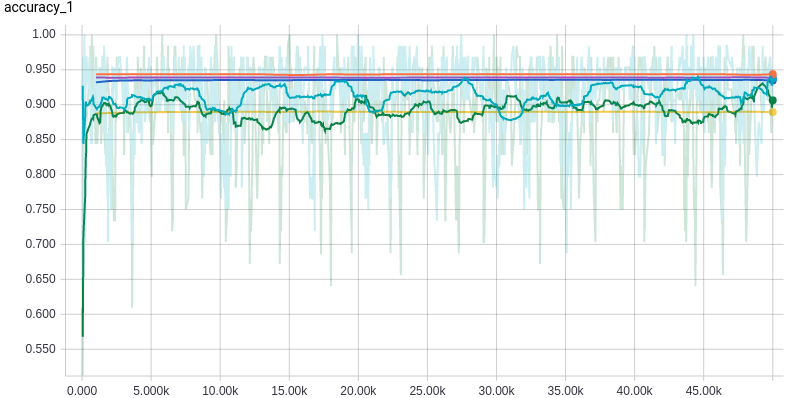
\includegraphics[width=\linewidth]{plots/model1/symmetrical/streak-r/accuracy.png}
    \caption{Accuracy using only rival streak.}\label{fig:symmetrical-r-accuracy}
  \end{subfigure}
  \begin{subfigure}{0.5\textwidth}
    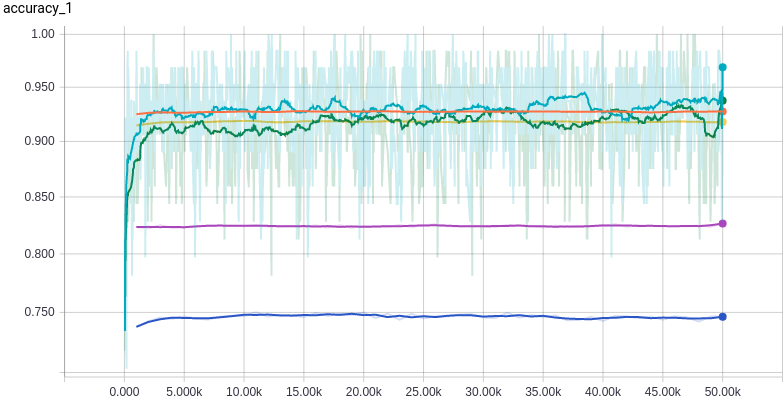
\includegraphics[width=\linewidth]{plots/model1/symmetrical/streak-hr/accuracy.png}
    \caption{Accuracy using both hot and rival streaks.}\label{fig:symmetrical-hr-accuracy}
  \end{subfigure}
  \caption{Accuracies for binary classification using the default (seasonal) temporal horizon.}
  \label{fig:symmetrical-accuracies}
\end{figure}

We can see that with a this model there is not a clear discrepancy between the compact and detailed datasets.
Though the respective curves (train, valid, test) exhibit the same behaviour, the compact-valid and detailed-test curves are significantly lower than their respective accuracy evaluation coutnerparts.

Note that the figures \ref{fig:symmetrical-r-accuracy} and \ref{fig:symmetrical-hr-accuracy} illustrate higher accuracies.
This is evidence that the rival streak is a good predictive feature.
It is also evident that the model can learn good parameter settings quickly with a steep ascend and plateauing around 3000 epochs, thereafter the model stalls and seems to be stuck in a local minimum.

Again, since all graphs do not overfit on either dataset, this suggests that the model is not flexible enough; however, the significantly poorer performance of the compact-valid and detailed-test curves seem to suggest that overfitting is occuring.



\begin{figure}[!htb]
  \begin{subfigure}{0.5\textwidth}
    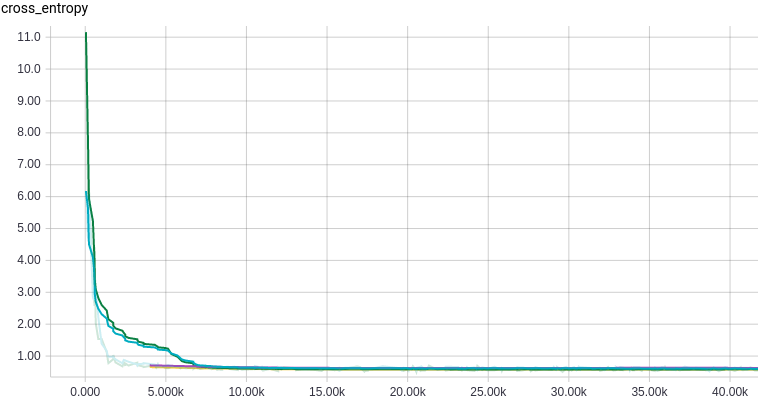
\includegraphics[width=\linewidth]{plots/model1/symmetrical/streak-/crossentropy.png}
    \caption{Cross Entropy using no streaks.}\label{fig:symmetrical--crossentropy}
  \end{subfigure}
  \begin{subfigure}{0.5\textwidth}
    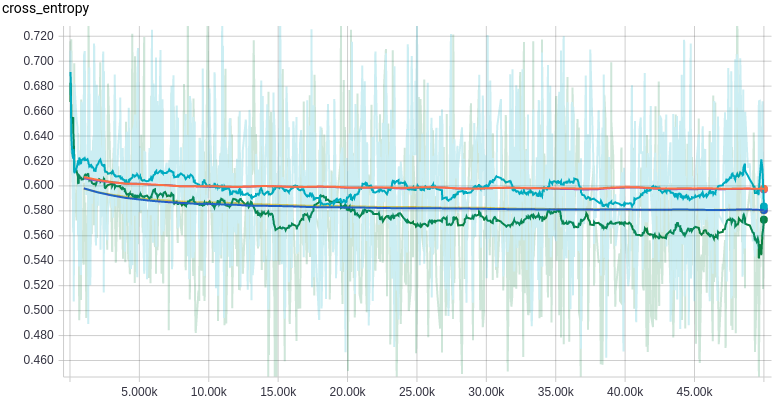
\includegraphics[width=\linewidth]{plots/model1/symmetrical/streak-h/crossentropy.png}
    \caption{Cross Entropy using only hot streak.}\label{fig:symmetrical-h-crossentropy}
  \end{subfigure}


  \begin{subfigure}{0.5\textwidth}
    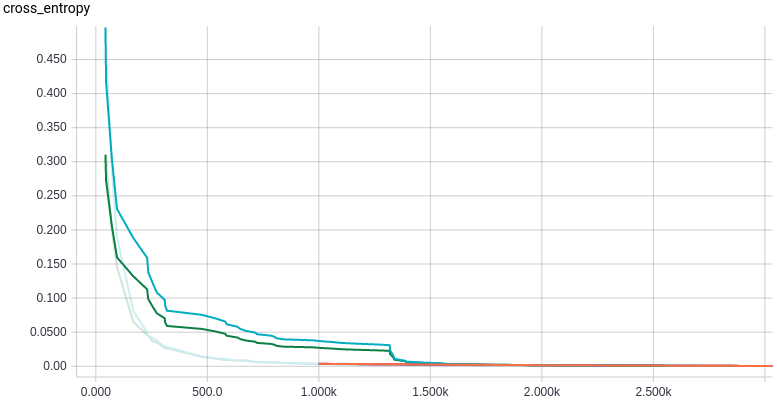
\includegraphics[width=\linewidth]{plots/model1/symmetrical/streak-r/crossentropy.png}
    \caption{Cross Entropy using only rival streak.}\label{fig:symmetrical-r-crossentropy}
  \end{subfigure}
  \begin{subfigure}{0.5\textwidth}
    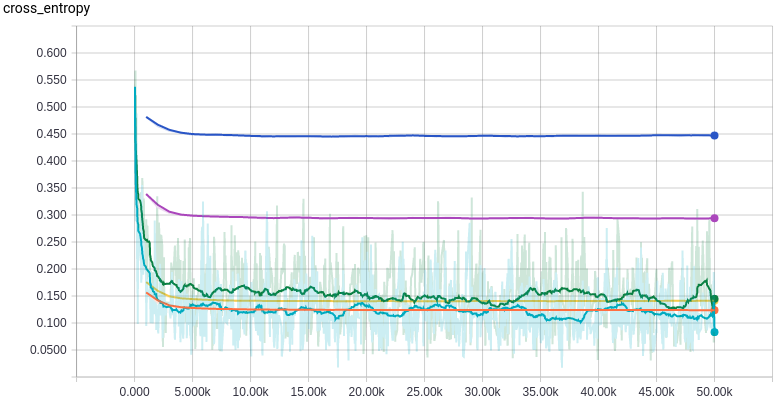
\includegraphics[width=\linewidth]{plots/model1/symmetrical/streak-hr/crossentropy.png}
    \caption{Cross Entropy using both hot and rival streaks.}\label{fig:symmetrical-hr-crossentropy}
  \end{subfigure}

  \caption{Cross Entropies for binary classification using the default (seasonal) temporal horizon.}
  \label{fig:symmetrical-crossentropies}
\end{figure}

The cross entropies are shown in figure~\ref{fig:symmetrical-crossentropies} where there does not seem to be any anomalies with respect to the corresponding accuracies.

Both input models that incorporate the rival streak have less loss as seen with higher accuracies in figure~\ref{fig:symmetrical-accuracies}.



\begin{table}
\centering
  \begin{tabular}{|l|c|c|c|c|}
  \hline
   & \multicolumn{2}{|c|}{Compact} & \multicolumn{2}{|c|}{Detailed}\\
  Data & loss & accuracy & loss & accuracy\\
  \hline
  Vanilla       & 0.6624 & 0.6094 & 0.5947 & 0.6871\\ 
  +hot streak   & 0.6425 & 0.6268 & 0.5935 & 0.6889\\
  +rival streak & 0.6340 & 0.6337 & 0.5897 & 0.6892\\
  +both streaks & 0.6339 & 0.6359 & 0.5910 & 0.6875\\
  \hline
  \end{tabular}
  \caption{Impact of the handcrafted streak features using the binary classification model.}
\end{table}
\label{tbl:test-results-symmetrical}

Table~\ref{tbl:test-results-symmetrical} shows that the binary classification problem produces a best accuracy $\approx 0.69$ which significantly outperforms the T-class classification problem above.
More interestingly, the detailed dataset significantly outperforms the compact dataset suggesting that at least one metric within this feature set adds significant predictive power.
Though hot and rival streaks add signifcant improvements to the compact featureset, their contribution is still present but borderline negligble when using the detailed feature set.
This does make sense though as there are significantly fewer games within the detailed dataset (which starts at year 2003 whereas compact dates back to 1985).
These streak features depend on a lot of data that is still not present if going back to 1985 and so the added improvement (though small) suggests that these streaks are good indicators for predicting game outcomes which significantly outperforms the T-class classification problem above.
More interestingly, the detailed dataset significantly outperforms the compact dataset suggesting that at least one metric within this feature set adds significant predictive power.
Though hot and rival streaks add signifcant improvements to the compact featureset, their contribution is still present but borderline negligble when using the detailed feature set.
This does make sense though as there are significantly fewer games within the detailed dataset (which starts at year 2003 whereas compact dates back to 1985).
These streak features depend on a lot of data that is still not present if going back to 1985 and so the added improvement (though small) suggests that these streaks are good indicators for predicting game outcomes.


\subsection{Investigating Different Temporal Horizons}
\label{sec:temporal-horizons}

The primary focus thus far has been on various feature combinations.
Using soley score in the compact dataset \ref{sec:data-features-compact} or the features in the detailed dataset \ref{sec:data-features-detailed}.

In this section we investigate using different temporal horizons.
Pairwise Matchups which aggregates the features based on all past games that two teams played against each other.
Secondly, we also look at liftime statistics which aggregates features based on all past games each team has played (not necessarily against one another).

\subsubsection{Lifetime Pairwise Matchups}

Lifetime pairwise matchups considers all past games where the two teams currently doing prediction on have played against each other and do not consider games where either team played a different team.



\begin{figure}[!htb]
  \begin{subfigure}{0.5\textwidth}
    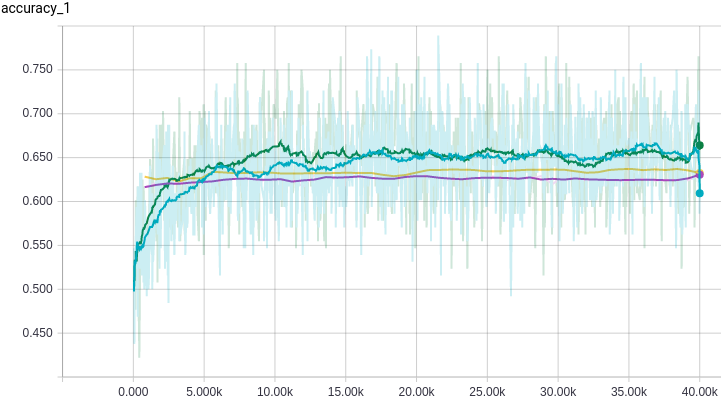
\includegraphics[width=\linewidth]{plots/model1/pairwise-matchups/streak-/accuracy.png}
    \caption{Accuracy using no streaks.}\label{fig:pairwise-matchups--accuracy}
  \end{subfigure}
  \begin{subfigure}{0.5\textwidth}
    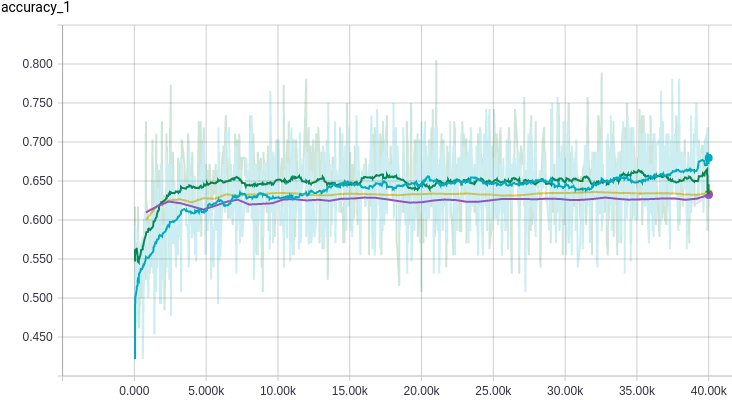
\includegraphics[width=\linewidth]{plots/model1/pairwise-matchups/streak-h/accuracy.png}
    \caption{Accuracy using only hot streak.}\label{fig:pairwise-matchups-h-accuracy}
  \end{subfigure}


  \begin{subfigure}{0.5\textwidth}
    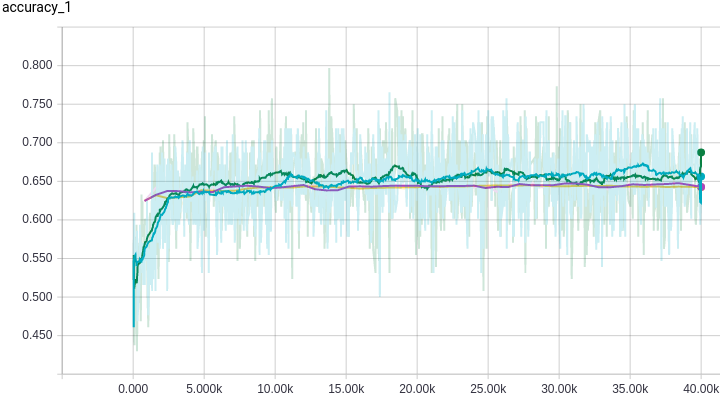
\includegraphics[width=\linewidth]{plots/model1/pairwise-matchups/streak-r/accuracy.png}
    \caption{Accuracy using only rival streak.}\label{fig:pairwise-matchups-r-accuracy}
  \end{subfigure}
  \begin{subfigure}{0.5\textwidth}
    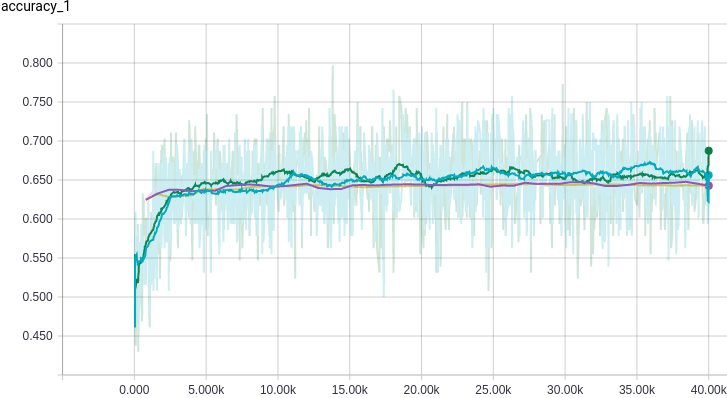
\includegraphics[width=\linewidth]{plots/model1/pairwise-matchups/streak-hr/accuracy.png}
    \caption{Accuracy using both hot and rival streaks.}\label{fig:pairwise-matchups-hr-accuracy}
  \end{subfigure}
  \caption{Accuracies using lifetime pairwise matchups as the temporal horizon.}
  \label{fig:pairwise-accuracies}
\end{figure}

We can see that with a this model there is not a clear discrepancy between the compact and detailed datasets.
This can be seen with all curves being close to one another with small to no gaps between them.
This is also supported in the test set in table~\ref{tbl:test-results-symmetrical-pairmatchups}.

Note that the figures \ref{fig:pairwise-matchups-r-accuracy} and \ref{fig:pairwise-matchups-hr-accuracy} illustrate higher accuracies.
This is evidence that the rival streak is a good predictive feature.
The inclusion of hot streak seems to add little benefit to the model.
This is evidenced by the loss and accuracy slighty decreasing and increasing respectively on both compact and detailed feature sets (though the loss actually increases by 0.0001 on compact.
Additionally, the composition of both streaks produce the best performance.
These are supported in table~\ref{tbl:test-results-symmetrical-pairmatchups} which lists the final loss and accuracy on the test set.

It is also evident that the model can learn good parameter settings quickly with a steep ascend and plateauing around 3000 epochs, thereafter the model stalls and seems to be stuck in a local minimum.

Again, since all graphs do not overfit on either dataset, this suggests that the model is not flexible enough; however, the significantly poorer performance of the compact-valid and detailed-test curves seem to suggest that overfitting is occuring.


\begin{figure}[!htb]
  \begin{subfigure}{0.5\textwidth}
    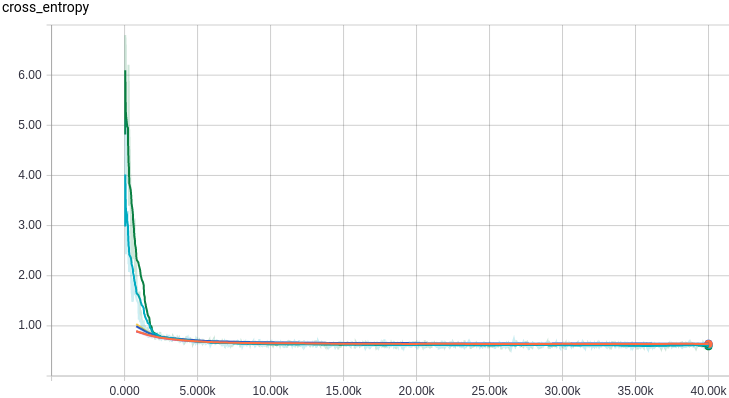
\includegraphics[width=\linewidth]{plots/model1/pairwise-matchups/streak-/crossentropy.png}
    \caption{Cross Entropy for pairwise matchups using no streaks.}\label{fig:pairwise--crossentropy}
  \end{subfigure}
  \begin{subfigure}{0.5\textwidth}
    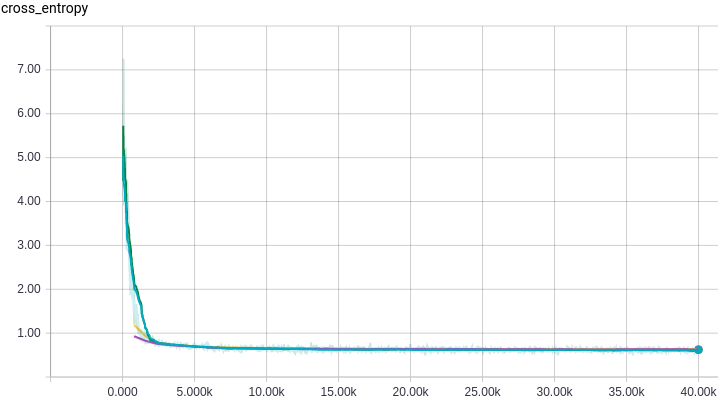
\includegraphics[width=\linewidth]{plots/model1/pairwise-matchups/streak-h/crossentropy.png}
    \caption{Cross Entropy for pairwise matchups using only hot streak.}\label{fig:pairwise-h-crossentropy}
  \end{subfigure}


  \begin{subfigure}{0.5\textwidth}
    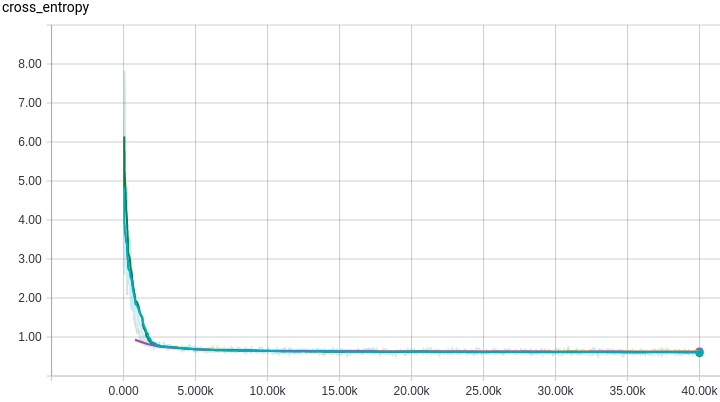
\includegraphics[width=\linewidth]{plots/model1/pairwise-matchups/streak-r/crossentropy.png}
    \caption{Cross Entropy for pairwise matchups using only rival streak.}\label{fig:pairwise-r-crossentropy}
  \end{subfigure}
  \begin{subfigure}{0.5\textwidth}
    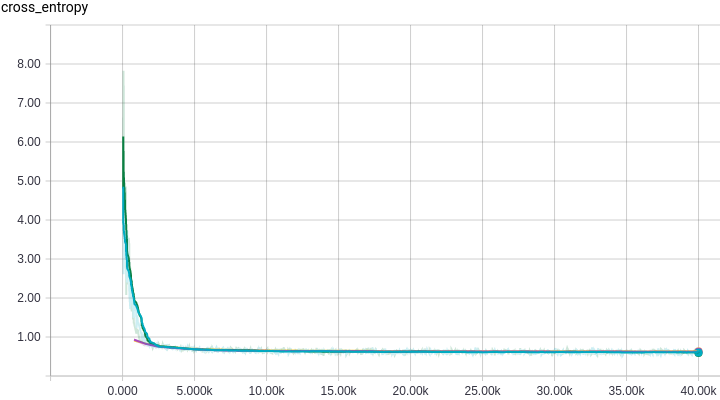
\includegraphics[width=\linewidth]{plots/model1/pairwise-matchups/streak-hr/crossentropy.png}
    \caption{Cross Entropy for pairwise matchups using both hot and rival streaks.}\label{fig:pairwise-hr-crossentropy}
  \end{subfigure}
  \caption{Cross Entropies using a lifetime pairwise matchup temporal horizon.}
  \label{fig:pairwise-crossentropies}
\end{figure}

The cross entropies are shown in figure~\ref{fig:pairwise-crossentropies} where there does not seem to be any anomalies with respect to the corresponding accuracies.

Both input models that incorporate the rival streak have less loss as seen with higher accuracies in figure~\ref{fig:pairwise-accuracies}.


\begin{table}
\centering
  \begin{tabular}{|l|c|c|c|c|}
  \hline
   & \multicolumn{2}{|c|}{Compact} & \multicolumn{2}{|c|}{Detailed}\\
  Data & loss & accuracy & loss & accuracy\\
  \hline
  Vanilla       & 0.6385 & 0.6187 & 0.6458 & 0.6228\\ 
  +hot streak   & 0.6386 & 0.6185 & 0.6447 & 0.6278\\
  +rival streak & 0.6414 & 0.6278 & 0.6404 & 0.6351\\
  +both streaks & 0.6395 & 0.6327 & 0.6437 & 0.6369\\
  \hline
  \end{tabular}
  \caption{Impact of the handcrafted streak features using the binary classification model using pairwise matchups for temporal horizon.}
\end{table}
\label{tbl:test-results-symmetrical-pairmatchups}

Table~\ref{tbl:test-results-symmetrical-pairmatchups} shows the performance on the test dataset using lifetime pairwise matchups as the temporal horizon.
The two feature sets are perform similarly with the detailed feature set slightly outperforming compact.



\subsubsection{Lifetime Statistics}

Lifetime statistics considers all past games where either team is playing.
The metrics for that game contribute to the metric for the team that is playing and averaged over the number of games each team has previously played.



\begin{figure}[!htb]
  \begin{subfigure}{0.5\textwidth}
    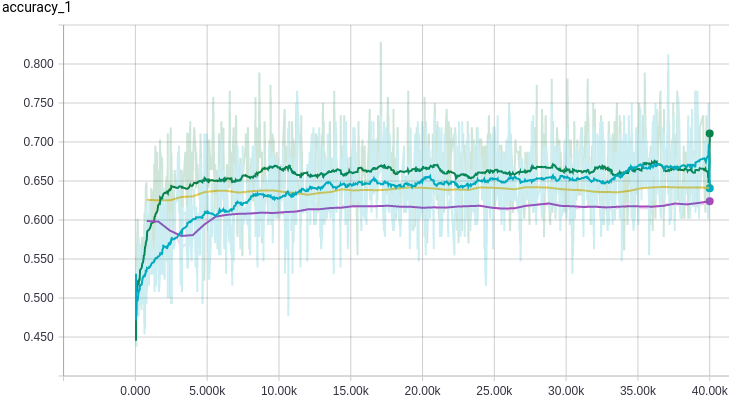
\includegraphics[width=\linewidth]{plots/model1/lifetime/streak-/accuracy.png}
    \caption{Accuracy using no streaks.}\label{fig:lifetime--accuracy}
  \end{subfigure}
  \begin{subfigure}{0.5\textwidth}
    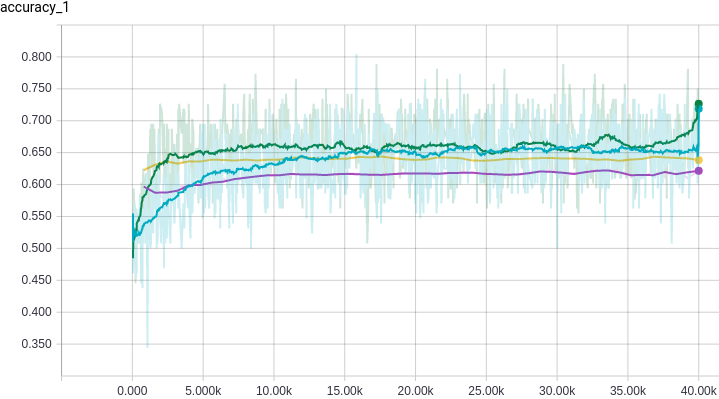
\includegraphics[width=\linewidth]{plots/model1/lifetime/streak-h/accuracy.png}
    \caption{Accuracy using only hot streak.}\label{fig:lifetime-h-accuracy}
  \end{subfigure}


  \begin{subfigure}{0.5\textwidth}
    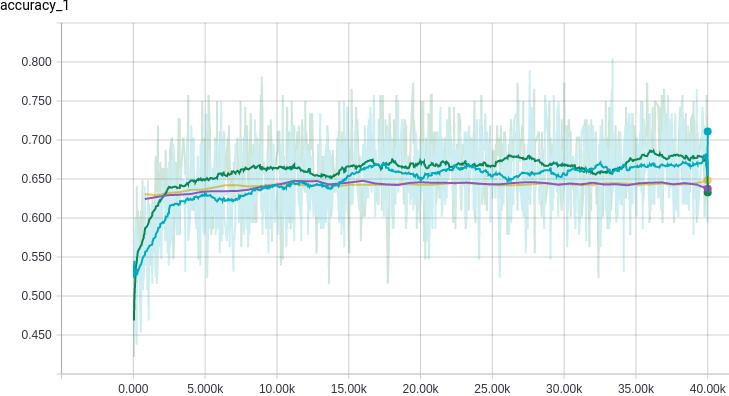
\includegraphics[width=\linewidth]{plots/model1/lifetime/streak-r/accuracy.png}
    \caption{Accuracy using only rival streak.}\label{fig:lifetime-r-accuracy}
  \end{subfigure}
  \begin{subfigure}{0.5\textwidth}
    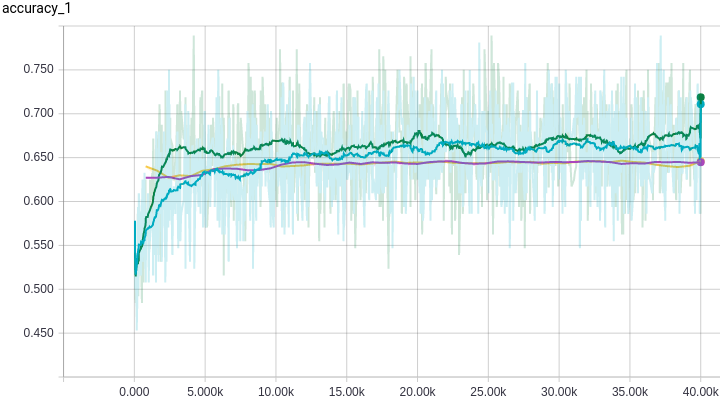
\includegraphics[width=\linewidth]{plots/model1/lifetime/streak-hr/accuracy.png}
    \caption{Accuracy using both hot and rival streaks.}\label{fig:lifetime-hr-accuracy}
  \end{subfigure}
  \caption{Accuracies using lifetime games as the temporal horizon.}
  \label{fig:lifetime-accuracies}
\end{figure}

We can see that with a this model there is not a clear discrepancy between the compact and detailed datasets.
Though the respective curves (train, valid) exhibit the same behaviour.

Note that the figures \ref{fig:lifetime-r-accuracy} and \ref{fig:lifetime-hr-accuracy} illustrate higher accuracies.
This is evidence that the rival streak is a good predictive feature.
However, the inclusion of hot streak seems to add confusion to the model and are not good predictors.
This is evidenced by the loss and accuracy slighty increasing and decreasing respectively on the detailed feature set.
Interestingly, for the compact feature set, rival streak seems to produce no benefits (with a minor performance degradation).
These are supported in table~\ref{tbl:test-results-symmetrical-lifetime} which lists the final loss and accuracy on the test set.

It is also evident that the model can learn good parameter settings quickly with a steep ascend and plateauing around 3000 epochs, thereafter the model stalls and seems to be stuck in a local minimum.

Again, since all graphs do not overfit on either dataset, this suggests that the model is not flexible enough; however, the significantly poorer performance of the compact-valid and detailed-test curves seem to suggest that overfitting is occuring.


\begin{figure}[!htb]
  \begin{subfigure}{0.5\textwidth}
    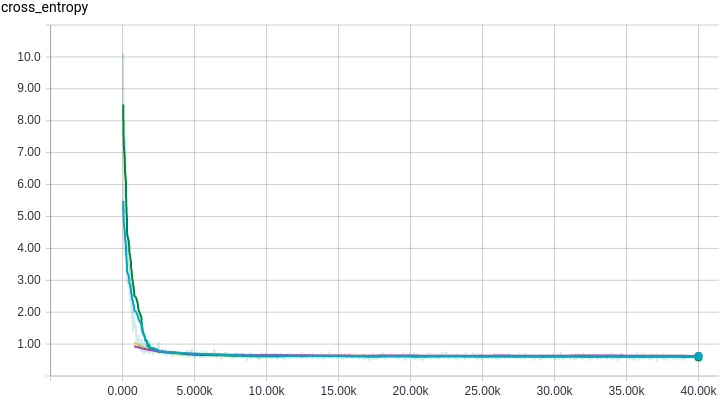
\includegraphics[width=\linewidth]{plots/model1/lifetime/streak-/crossentropy.png}
    \caption{Cross Entropy across lifetime games using no streaks.}\label{fig:lifetime--crossentropy}
  \end{subfigure}
  \begin{subfigure}{0.5\textwidth}
    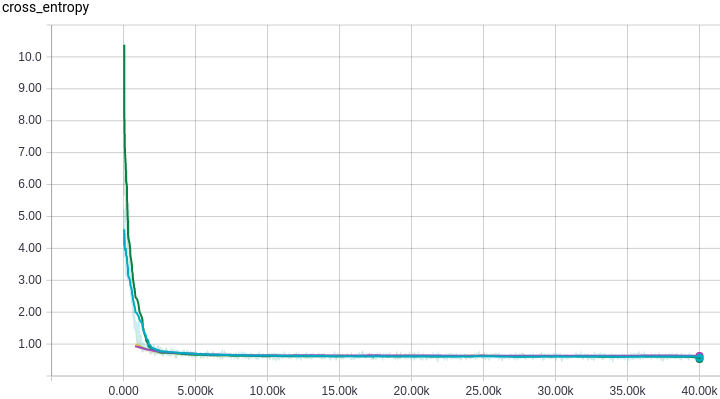
\includegraphics[width=\linewidth]{plots/model1/lifetime/streak-h/crossentropy.png}
    \caption{Cross Entropy across lifetime games using only hot streak.}\label{fig:lifetime-h-crossentropy}
  \end{subfigure}


  \begin{subfigure}{0.5\textwidth}
    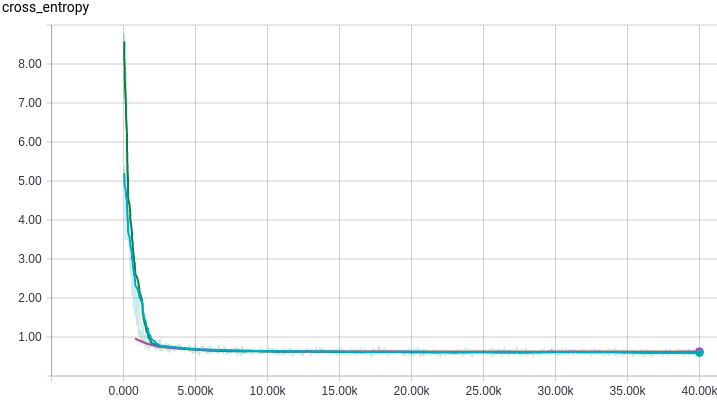
\includegraphics[width=\linewidth]{plots/model1/lifetime/streak-r/crossentropy.png}
    \caption{Cross Entropy across lifetime games using only rival streak.}\label{fig:lifetime-r-crossentropy}
  \end{subfigure}
  \begin{subfigure}{0.5\textwidth}
    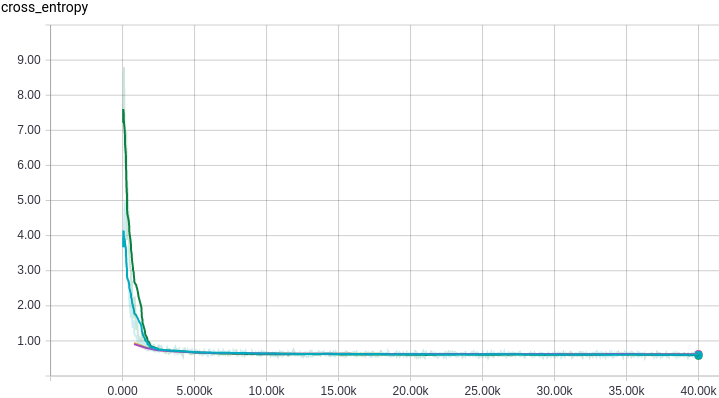
\includegraphics[width=\linewidth]{plots/model1/lifetime/streak-hr/crossentropy.png}
    \caption{Cross Entropy across lifetime games using both hot and rival streaks.}\label{fig:lifetime-hr-crossentropy}
  \end{subfigure}
  \caption{Cross Entropies using lifetime games as the temporal horizon.}
  \label{fig:lifetime-crossentropies}
\end{figure}

The cross entropies are shown in figure~\ref{fig:lifetime-crossentropies} where there does not seem to be any anomalies with respect to the corresponding accuracies.

Both input models that incorporate the rival streak have less loss as seen with higher accuracies in figure~\ref{fig:lifetime-accuracies}.


\begin{table}
\centering
  \begin{tabular}{|l|c|c|c|c|}
  \hline
   & \multicolumn{2}{|c|}{Compact} & \multicolumn{2}{|c|}{Detailed}\\
  Data & loss & accuracy & loss & accuracy\\
  \hline
  Vanilla       & 0.6418 & 0.6143 & 0.6371 & 0.6355\\ 
  +hot streak   & 0.6425 & 0.6144 & 0.6372 & 0.6343\\
  +rival streak & 0.6492 & 0.6211 & 0.6314 & 0.6408\\
  +both streaks & 0.6414 & 0.6272 & 0.6316 & 0.6377\\
  \hline
  \end{tabular}
  \caption{Impact of the handcrafted streak features using the binary classification model using lifetime statistics for temporal horizon.}
\end{table}
\label{tbl:test-results-symmetrical-lifetime}

Table~\ref{tbl:test-results-symmetrical-lifetime} shows the performance on the test dataset using lifetime statistics as the temporal horizon.
The detailed feature set outperforms compact.


\subsection{Neural Network with 2 Hidden Layers}

We investigate adding complexity to the NN model by adding an additional hidden layer.
A seasonal temporal horizon is used as it performs the best which is evidenced in temporal horizon experiments in section~\ref{sec:temporal-horizons}.



\begin{figure}[!htb]
  \begin{subfigure}{0.5\textwidth}
    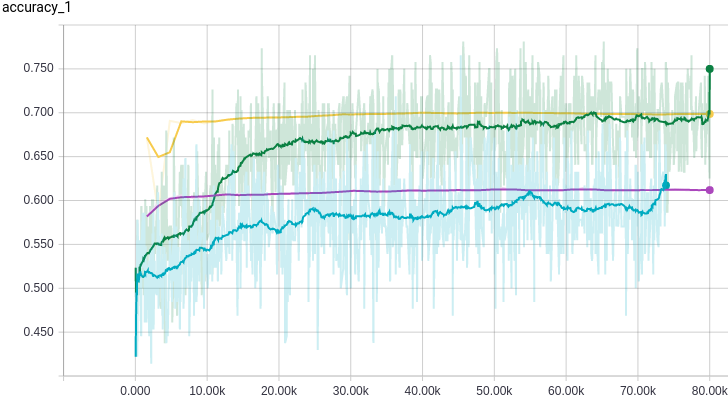
\includegraphics[width=\linewidth]{plots/model2/streak-/accuracy.png}
    \caption{Accuracy using no streaks.}\label{fig:model2--accuracy}
  \end{subfigure}
  \begin{subfigure}{0.5\textwidth}
    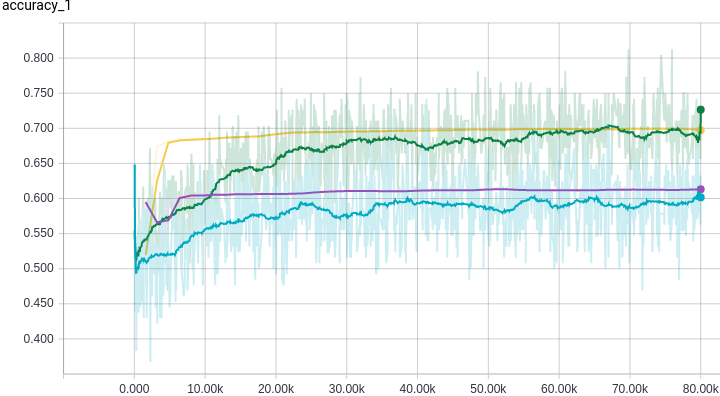
\includegraphics[width=\linewidth]{plots/model2/streak-h/accuracy.png}
    \caption{Accuracy using only hot streak.}\label{fig:model2-h-accuracy}
  \end{subfigure}


  \begin{subfigure}{0.5\textwidth}
    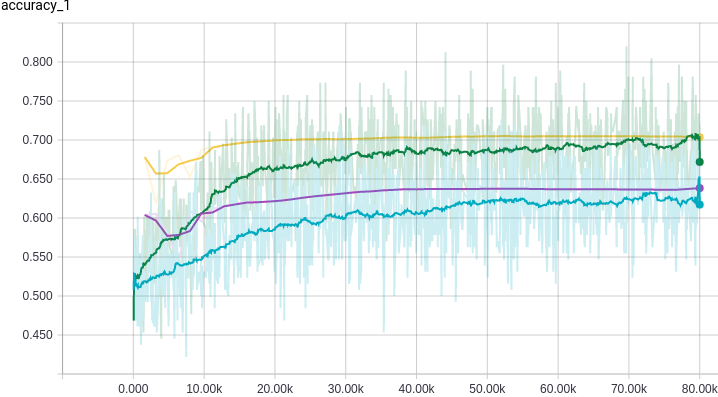
\includegraphics[width=\linewidth]{plots/model2/streak-r/accuracy.png}
    \caption{Accuracy using only rival streak.}\label{fig:model2-r-accuracy}
  \end{subfigure}
  \begin{subfigure}{0.5\textwidth}
    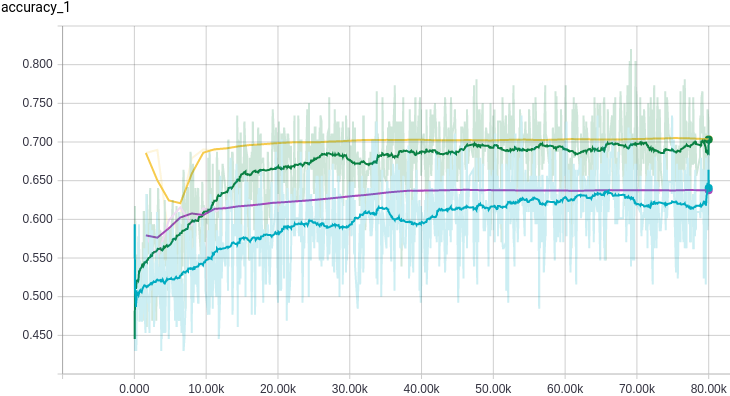
\includegraphics[width=\linewidth]{plots/model2/streak-hr/accuracy.png}
    \caption{Accuracy using both hot and rival streaks.}\label{fig:model2-hr-accuracy}
  \end{subfigure}
  \caption{Accuracies using seasonal games with a neural network with two hidden layers.}
  \label{fig:model2-accuracies}
\end{figure}

We can see that with a this model there is a clear discrepancy between the compact and detailed datasets (which seems to be attributed to the choice of a temporal horizon [seasonal games]).

Note that the figures \ref{fig:model2-r-accuracy} and \ref{fig:model2-hr-accuracy} illustrate higher accuracies (for the compact feature set).
This is evidence that the rival streak is a good predictive feature but not as useful when combines with the features in the detailed features.
The model gradually learns good parameter settings compared to the single hidden layer model (as there are more paramters to tune).

Again, since all graphs do not overfit on either dataset, this suggests that the model is not flexible enough; however, the significantly poorer performance of the compact-valid and detailed-test curves seem to suggest that overfitting is occuring.



\begin{figure}[!htb]
  \begin{subfigure}{0.5\textwidth}
    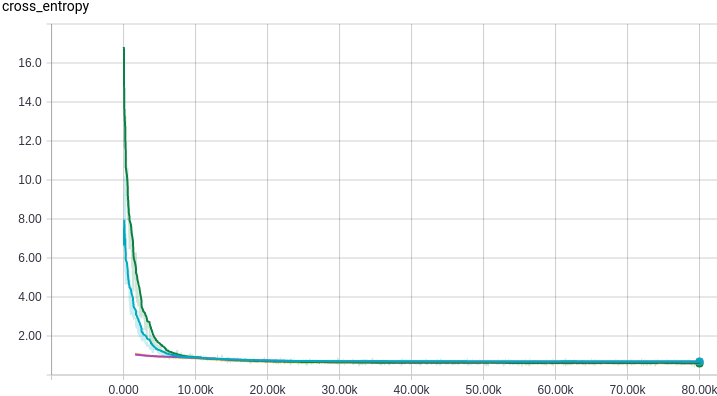
\includegraphics[width=\linewidth]{plots/model2/streak-/crossentropy.png}
    \caption{Cross Entropy using no streaks.}\label{fig:model2--crossentropy}
  \end{subfigure}
  \begin{subfigure}{0.5\textwidth}
    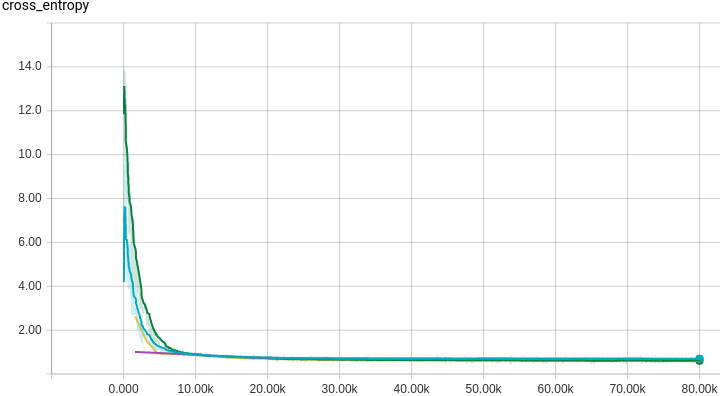
\includegraphics[width=\linewidth]{plots/model2/streak-h/crossentropy.png}
    \caption{Cross Entropy using only hot streak.}\label{fig:model2-h-crossentropy}
  \end{subfigure}


  \begin{subfigure}{0.5\textwidth}
    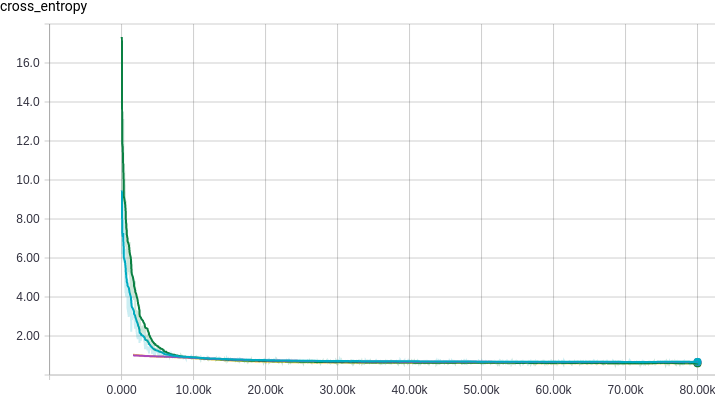
\includegraphics[width=\linewidth]{plots/model2/streak-r/crossentropy.png}
    \caption{Cross Entropy using only rival streak.}\label{fig:model2-r-crossentropy}
  \end{subfigure}
  \begin{subfigure}{0.5\textwidth}
    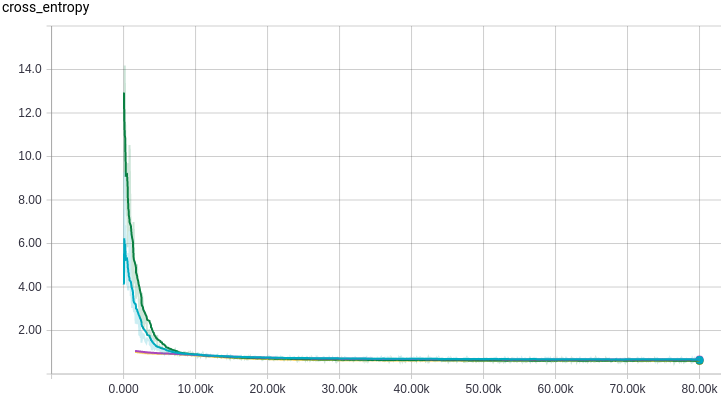
\includegraphics[width=\linewidth]{plots/model2/streak-hr/crossentropy.png}
    \caption{Cross Entropy using both hot and rival streaks.}\label{fig:model2-hr-crossentropy}
  \end{subfigure}
  \caption{Cross Entropies using seasonal games with a neural network with two hidden layers.}
  \label{fig:model2-crossentropies}
\end{figure}

The cross entropies are shown in figure~\ref{fig:model2-crossentropies} where there does not seem to be any anomalies with respect to the corresponding accuracies.

Both input models that incorporate the rival streak have less loss as seen with higher accuracies in figure~\ref{fig:model2-accuracies}.

\begin{table}
\centering
  \begin{tabular}{|l|c|c|c|c|}
  \hline
   & \multicolumn{2}{|c|}{Compact} & \multicolumn{2}{|c|}{Detailed}\\
  Data & loss & accuracy & loss & accuracy\\
  \hline
  Vanilla       & 0.6924 & 0.6003 & 0.6201 & 0.6869\\ 
  +hot streak   & 0.6923 & 0.6007 & 0.6193 & 0.6867\\
  +rival streak & 0.6678 & 0.6346 & 0.6176 & 0.6876\\
  +both streaks & 0.6683 & 0.6339 & 0.6179 & 0.6871\\
  \hline
  \end{tabular}
  \caption{Impact of the handcrafted streak features using the binary classification model on a NN with 2 hidden layers.}
\end{table}
\label{tbl:test-results-symmetrical-2hiddenlayers}

Table~\ref{tbl:test-results-symmetrical-2hiddenlayers} shows the performance on the test dataset using seasonal temporal horizon on a neural network with 2 hidden layers.
Analogous to table~\ref{tbl:test-results-symmetrical} the performances are similar where adding an extra layer hinders the performance on the compact feature set but improves the performance on the detailed feature set.



\section{Investigating Temporal Correlations for RNNs}

\textbf{Investigating Rival Streak Correlation}
Data was aggregated with rival streak encompassing the entire feature space.
Some inquisitions lead us to investigate whether or not providing the rival streak was leaking data to the model since the input of some examples contained the output of others.
However, since each example was computed solely on temporal historical data, there should be no data leaking.

It then seemed natural that the rival streak values were highly correlated, so we investigated the covariance matrix:

\if false
\[
\begin{bmatrix}
  0.50134639 &  0.         &  0.         &  0.         &  0.         &
  0.         &  0.         &  0.         & 0.          &  0.        \\
  0.         &  0.7500612  &  0.         &  0.00097919 &  0.00097919 &
  0.         & -0.00097919 & -0.00097919 &  0.00097919 &  0.        \\
  0.         &  0.         &  0.8753978  &  0.00097919 &  0.00097919 &
  0.         &  0.00097919 & -0.00097919 & -0.00097919 &  0.        \\
  0.         &  0.00097919 &  0.00097919 &  0.9380661  &  0.         &
  -0.00097919 &  0.         &  0.00195838 &  0.         & -0.00097919\\
  0.         &  0.00097919 &  0.00097919 &  0.         &  0.96940024 &
  0.00097919 &  0.         &  0.         &  0.         &  0.00097919\\
  0.         &  0.         &  0.         & -0.00097919 &  0.00097919 &
  0.98506732 & -0.00097919 &  0.00097919 &  0.00097919 &  0.        \\
  0.         & -0.00097919 &  0.00097919 &  0.         &  0.         &
  -0.00097919 &  0.99290086 &  0.         &  0.00195838 &  0.00097919\\
  0.         & -0.00097919 & -0.00097919 &  0.00195838 &  0.         &
  0.00097919 &  0.         &  0.99681763 &  0.         &  0.00097919\\
  0.         &  0.00097919 & -0.00097919 &  0.         &  0.         &
  0.00097919 &  0.00195838 &  0.         &  0.99877601 & -0.00097919\\
  0.         &  0.         &  0.         & -0.00097919 &  0.00097919 &
  0.         &  0.00097919 &  0.00097919 & -0.00097919 &  0.9997552
\end{bmatrix}
\]
\fi


\[
\begin{bmatrix}
  0.5013 &  0.     &  0.     &  0.     &  0.     &  0.     &  0.     &  0.     &  0.     &  0.    \\
  0.     &  0.7501 &  0.     &  0.0010 &  0.0010 &  0.     & -0.0010 & -0.0010 &  0.0010 &  0.    \\
  0.     &  0.     &  0.8754 &  0.0010 &  0.0010 &  0.     &  0.0010 & -0.0010 & -0.0010 &  0.    \\
  0.     &  0.0010 &  0.0010 &  0.9381 &  0.     & -0.0010 &  0.     &  0.0200 &  0.     & -0.0010\\
  0.     &  0.0010 &  0.0010 &  0.     &  0.9694 &  0.0010 &  0.     &  0.     &  0.     &  0.0010\\
  0.     &  0.     &  0.     & -0.0010 &  0.0010 &  0.9851 & -0.0010 &  0.0010 &  0.0010 &  0.    \\
  0.     & -0.0010 &  0.0010 &  0.     &  0.     & -0.0010 &  0.9929 &  0.     &  0.0200 &  0.0010\\
  0.     & -0.0010 & -0.0010 &  0.0200 &  0.     &  0.0010 &  0.     &  0.9968 &  0.     &  0.0010\\
  0.     &  0.0010 & -0.0010 &  0.     &  0.     &  0.0010 &  0.0020 &  0.     &  0.9988 & -0.0010\\
  0.     &  0.     &  0.     & -0.0010 &  0.0010 &  0.     &  0.0010 &  0.0010 & -0.0010 &  0.9998
\end{bmatrix}
\]
Though there is evidence of some minor correlation, the values are lower than anticipated.


\section{Data Interpretation}
\label{sec:data-interpretation}

Convolutional neural networks allow gradient ascent to view visualizations of the filters that are learned to better interpret what the modelis learning.
In a MLP there is nothing similar that can be done aside from presenting visualizations of the predictions.

To better understand the probabilities between teams with the ultimate goal of determining bracketology we helped develop a visualization that will execute a complete bracket if given the first round teams and seeds.

The code is at \citep{bracket-visual} and an example output for the 2017 March Madness prediction is in figure~\ref{fig:bracket-visual}.
Though it is not complete, it presents the information the user cares about (which the user can decide by inputting their own team-seed mapping).

\begin{figure}[!htb]
  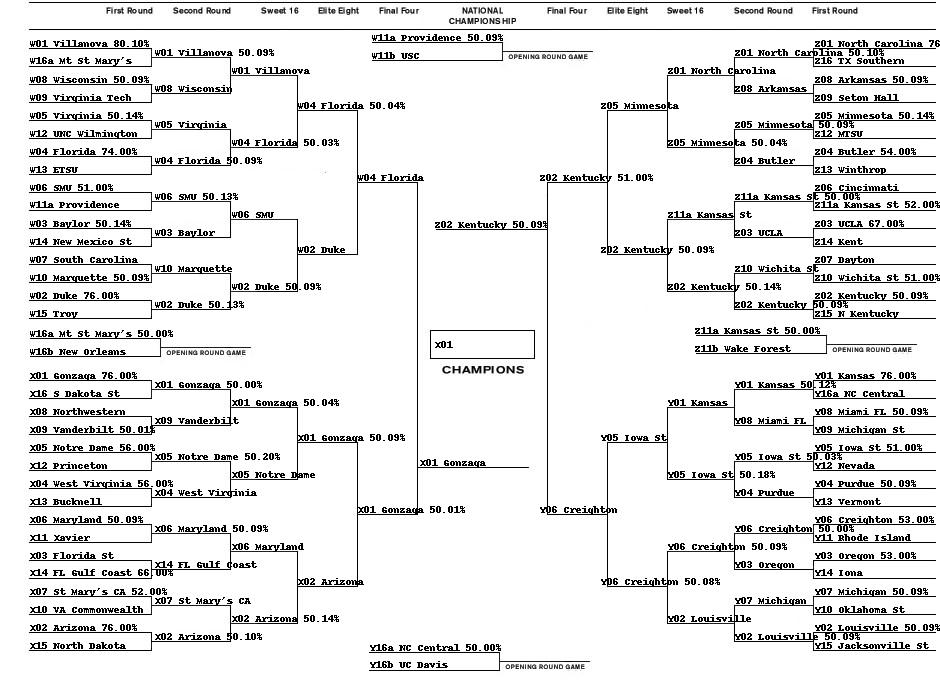
\includegraphics[width=\linewidth]{figures/predicted-bracket.jpg}
  \caption{Example visualization of a bracket which uses model-generated probabilities to complete the bracket.}
  \label{fig:bracket-visual}
\end{figure}


\section{Conclusion}
\label{sec:conclusion}

The results suggest that using a seasonal temporal horizon best indicates the winning team.
Additionally, across all models, the handcrafted features (hot and rival streak) add useful information for the model to better predict (slightly) the outcome of a NCAA basketball game.
Expectedly, the multi-class model performs worse than the binary classification model but does perform quite well considering it must learn valid outputs.

Throughout most models including rival streak increases performance.
Adding complexity throught he use of NNs slightly improves over the logistic baseline (the best configurations having a difference less than $1\%$) suggesting that adding additionaly complexity is probably not the best way to construct a good general model.

The loss figures each model suggest that no model investigated is appropriate for this domain.
Some NN configurations were ran for 200k epochs (instead of the 80k presented) to get a better sense if the model were to ever overfit on the training data.
This never occurred.
Normally, you want to stop training at a point where the training loss is increasing and the validation has reached a peak and has begun to descend again (a large enough peak so that it is not due to small perturbations) suggesting t the model is beginning to overfit the training data and was previously in a good ``generalized" configuration.
Since this never occured in any model/configuration combination, none of the models investigated were good for this domain (or the domain may be hard which is possible for game outcomes).

Furthermore, seasonal temporal horizon outperformed both lifetime statistic and lifetime previous game matchups which was expected.
Seasonal games give teams a fresh start for when their verteran players graduate school and new players come in to their roster---potentially leaving a brand new team unlike the previous year.
If this were NBA then maybe using one of the lifetime horizons would be better suited.
One pitfall is with the amount of data---with rival streak performing quite well even though many team matchups are not present in the current data this suggests that if more data were available the impact of rival streak could be even greater.


Additionally, we chose to abstract bracketology to simple game predictions.
A subtle but important difference should be noted---momentum.
In tournaments, some ``underdog" teams manage to go on a win (hot) streak after defeating one of the highest seeds team and result in more upsets.
We do not account for any such momentum or even seeds.
This could, probably, improve the performance but we are uncertain.


Other ways of performing bracketology instead of an exponential scoring system that is used is to re-run your predictions after each round (this will allow models to better incorporate momentum as each round finishes in the unlikely event of an upset).




\small{
\nocite{*}
\bibliographystyle{plainnat}
\bibliography{research}
}
\end{document}
